% !TEX root = ../main.tex

\begin{savequote}[99mm]
Some people would claim that things like love, joy and beauty belong to a different category from science and can't be described in scientific terms, but I think they can now be explained by the theory of evolution.
\qauthor{Stephen Hawking}
\end{savequote}

\chapter{Evolutionary solution to the identification problem}
\label{chap:id-bin}

In this chapter we describe the solution of the identification problem, for which an evolutionary algorithm based on a GA~\cite{holland1975adaptation} will be used. GAs constitute a  well-known optimization method used in many domains of application, including earlier research on CAs. For example,
GAs have been used in the construction of CA-based random number generators~\cite{TOMASSINI2001151}, for finding CAs capable of image reconstruction~\cite{Seredynski2012} and for retrieving CA-based population models of competing individuals~\cite{Schimit2014}.

For the sake of reproducibility, we formally define the GA by clearly giving the individuals' representation, structure of the population, a fitness function, the genetic operators, namely the selection procedure for reproduction, and the cross-over and mutation operators, and finally the halting conditions.

\section{Individuals and populations}
Here, the individuals that make up the population are CAs, encoded through the LUT of their local rule, which is possible since the LUT of any CA $A\in\mathcal{A}_r$ can be represented as a bit-string of length $2^{2\,r+1}$ (see Section~\ref{sec:prem}).

The population is a collection of local rules with different radii between $r_{\ast}$ and~$r^{\ast}$, since the radius of the desired solution might not be known in practice and one of the goals is to detect it. Note that as a consequence of Fact~\ref{fac:incl}, we might opt to consider populations of local rules with radius $r^{\ast}$ only, but by allowing diverse radii, populations can evolve quicker and produce simpler solutions, \emph{i.e.}\ local rules with smaller radii.

The number of CAs in a population is denoted by $P>0$. The symbol $\mathcal{P}^n$, where $n=1,2,\dotsc$, denotes the population of the $n$-th generation of the GA. Population $\mathcal{P}^1$ is the initial population, and is constructed by randomly selecting $P$ bit-strings. Let $\mathcal{P}^1 = \{L^1_1,\dotsc,L^1_P\}$, where $L^1_i$ is the $i$-th individual in the initial population, then $\abs{L^1_i} = 2^{2\,r_i+1}$ for some $r_i\in\{r_{\ast},\dotsc,r^{\ast}\}$. This radius $r_i$ can change as the GA evolves. Populations $\mathcal{P}^n$ for $n>1$ are evolved by applying the genetic operators described in the remainder of this section. Individuals belonging to the $n$-th population are denoted by $L^n_i$, for $i=1,\dotsc,P$.

\section{Fitness function}\label{sec:fitness}
The fitness function is directly related to the error measure $\widetilde{E}_{\mathcal{I}}$ defined by~\eqref{eq:error}.
% Although Proposition~\ref{fac:relationoferror} states that the error measures given by~\eqref{eq:error0} and~\eqref{eq:error} can be used interchangeably, preliminary experiments showed that the latter results in an efficient and convergent algorithm, while suboptimal results were obtained using the measure given by~\eqref{eq:error0}. This follows from the fact that the error in row $n$ is affected by errors appearing in rows $2,\dotsc,n-1$. As we know from the research on dynamical properties of CAs that small initial perturbations can strongly affect further system states\cite{jan.lyap}, it is easier to optimize $\widetilde{E}_{\mathcal{I}}$ with a GA than $E_{\mathcal{I}}$. 
Let $L\in\{0,1\}^{2^{2\,r+1}}$ be the LUT of some local rule that defines a CA $A$. Then $\fit_{\mathcal{I}}(L)$ denotes the fitness of $A$, and is defined as:
\begin{equation}
	\fit_{\mathcal{I}}(L) = C(\mathcal{I}) - M_\mathcal{I} - \widetilde{E}_\mathcal{I}(A)\,.
	\label{eq:fit-org}
\end{equation}
The fitness function takes integer values from 0 up to $C(\mathcal{I}) - M_\mathcal{I}$ which is the total number of completely observed states excluding the states in all of the initial configurations. Therefore, there are only finitely many values of the fitness function. The goal of the GA is to maximize fitness, and a CA leading to maximal fitness is a solution of the identification problem.
From the above, it is relatively clear that if $C(\mathcal{I}) - M_\mathcal{I}$ (the number of completely observed cells not counting the first rows) is close to zero then the problem is not very interesting. 
Additionally, if $C(\mathcal{I}) = M_\mathcal{I}$, then the problem is trivial because every CA is a solution.

Initial experiments have shown that the fitness function defined by~\eqref{eq:fit-org} is effective. Yet, the computing time for finding its values is unacceptable when large observation sets are considered, since the cost of computing an exact value is linear in the size of the observation set. An approximation algorithm is used to overcome this issue for a large observation set. During the evolution of the $n$-th population, we estimate the value of $\fit_{\mathcal{I}}$ by using $\fit_{\mathcal{I}_n}$, where $\mathcal{I}_n\subset\mathcal{I}$ is a non-empty subset. Such an approach is justified by Fact~\ref{fac:rules-set}, which assures that the solution set is not being reduced. The set $\mathcal{I}_1$ is a subset of $0<s\leq \abs{\mathcal{I}}$ randomly selected observations of $\mathcal{I}$, while the set $\mathcal{I}_{n+1}$, for $n\geq 1$, is built from $\mathcal{I}_{n}$ by replacing one of its observations denoted by $I_r$, with a new selection from $\mathcal{I} \backslash \mathcal{I}_{n}$ denoted by $I_a$. There are two scenarios for selecting~$I_r$ and~$I_a$, depending on the contents of $\mathcal{I}_n$, which are presented below.

Let $B(n)$ yield the fittest individual from the $n$-th population, {\it i.e.}\
\begin{equation}
	B(n) = \argmax_{L\in\mathcal{P}^{n}} \fit_{\mathcal{I}_{n}}(L)\,.
\end{equation}
If multiple choices of $B(n)$ are possible, we pick one at random.
As described in more detail in Section~\ref{sec:halt}, for such an individual, the fitness $\fit_{\mathcal{I}}$ over the entire set $\mathcal{I}$ is recalculated verifying  whether the halting condition is satisfied at every iteration of the GA. Consequently, we have access to the values $\widetilde{E}_I(B(n))$ for any $I\in\mathcal{I}$, and thus we can easily find $I^{\ast}\in\mathcal{I}$ such that $\widetilde{E}_{I^{\ast}}(B(n)) \geq \widetilde{E}_I(B(n))$ for any $I\in\mathcal{I}$.

If $I^{\ast} \in \mathcal{I}_{n}$, then $I_r$ is selected randomly from $\mathcal{I}_{n}$ in such a way that $I_r \neq I^{\ast}$ and $I_a$ is also selected randomly from $\mathcal{I}\backslash \mathcal{I}_{n}$. On the other hand, if $I^{\ast} \not\in \mathcal{I}_{n}$, then $I_a = I^{\ast}$ and~$I_r$ is selected randomly from $\mathcal{I}_{n}$. Formally, the goal of this procedure is to assure that the observation resulting in the highest error $I^{\ast}$ is included in $\mathcal{I}_{n+1}$ and that exactly one observation is replaced at every generation, \emph{i.e.}\ $\abs{\mathcal{I}_{n} \cap \mathcal{I}_{n+1}} = s-1$.
In Algorithm~\ref{algo:ga}, we use $\Fbuildset{$\mathcal{I}_n, E^n$}$ to denote the subset $\mathcal{I}_{n+1}$ obtained according to the procedure outlined above. The argument $E^n$ corresponds to the error vector of the individual $B(n)$, \emph{i.e.}\ $E^n = \big(\widetilde{E}_I(B(n))\big)_{I\in\mathcal{I}}$. Further, $\Ferrorvec{$L, \mathcal{I}$}$ denotes a function that returns a vector of the form $(\widetilde{E}_{I}(L))_{I\in\mathcal{I}}$.

Let $F(n)$ denote the highest fitness observed among the individuals that had the highest values of fitness estimation during the GA evolution up to the $n$-th generation. Let $n\in\mathbb{N}$, then $F(n)$ is defined as $F(n) = \max_{i\in\{1,\dotsc,n\}} \fit_{\mathcal{I}}\left(B(i)\right)$.

Obviously $F(n)\leq F(n+1)$. In addition to this maximal fitness $F$, we also define the age of this value as the number of GA iterations during which the maximal fitness did not change. Formally, a value $F(n)$ has an age $a(n)>0$ if and only if it holds that:
\[F(n-a(n)-1) < F(n-a(n)) = \cdots = F(n-1) = F(n)\,.\]

\section{Selection}\label{sec:select}
% Here we define the selection operator. It is used for selecting the parent individuals for reproduction. 
We use a standard, random selection method. The probability of selecting a given individual is proportional to its fitness. This is feasible, since the fitness function introduced in Section~\ref{sec:fitness} is bounded. The selection process is repeated with replacement, so that each of the individuals can be selected multiple times.
In the pseudo-code, the function $\selectParents{$\mathcal{P}$}$ returns two individuals selected from population $\mathcal{P}$ according to this selection procedure.

\section{LUT rescaling}\label{sec:rescal}
Before describing the cross-over operator, we introduce a rescaling operation in order to be able to define cross-over of LUTs with different radii. Given Fact~\ref{fac:incl}, each CA defined by a local rule with neighborhood radius $r$, can also be defined by a local rule with neighborhood radius $r+1$. A simple method for ``converting'' the LUT of a given local rule $f$, with radius $r$, to the LUT of its corresponding local rule $f^\uparrow$, with radius $r+1$, follows from the fact $f^\uparrow(s_1, \dotsc, s_{2\,(r+1)+1}) = f(s_2,\dotsc,s_{2\,r+2})$, for all $s_1,\dotsc,s_{2\,(r+1)+1}\in\{0,1\}$. Note that both $f$ and $f^\uparrow$ define the same CA. The operation of increasing the radius by one will be referred to as up-scaling by one. Let $L\in\{0,1\}^{2^{2\,r+1}}$ be the LUT of $f$, then the LUT of $f^\uparrow$, denoted as $L^\uparrow\in\{0,1\}^{2^{2(r+1)+1}}$, can be constructed from $L$ using Algorithm~\ref{algo:up}.

\begin{figure}[!t]
	\removelatexerror\begin{algorithm}[H]
		\KwIn{LUT given by variable $L$.}
		\KwOut{Up-scaled LUT stored in variable $L^\uparrow$.}
		\For{$i=1,\dotsc,2^{2\,r+1}$}{
		$L^\uparrow[2\,i] \gets L[i]$\;
		$L^\uparrow[2\,i-1] \gets L[i]$\;
		$L^\uparrow[2\,i-1+2^{2\,r+2}] \gets L[i]$\;
		$L^\uparrow[2\,i+2^{2\,r+2}] \gets L[i]$\;
		}
		\caption{Up-scaling of the LUT}\label{algo:up}
	\end{algorithm}
\end{figure}

Similarly to the up-scaling operation, we define the inverse operation. Let $f$ be a local rule with neighborhood radius $r$, then the down-scaled local rule $f_\downarrow$, with radius $r-1$, is defined as:
\begin{equation*}
	f_\downarrow(s_1,\dotsc,s_{2\,r-1}) = \left[\frac{1}{4}\sum_{a=0}^{1}\sum_{b=0}^{1}f(a,s_1,\dotsc,s_{2\,r-1},b)\right],
\end{equation*}
where $[\cdot]$ indicates rounding to the nearest integer (we assume $[0.5]=0$). The method of computing the LUT of the down-scaled rule is presented in Algorithm~\ref{algo:down}. Let $L\in\{0,1\}^{2^{2\,r+1}}$ be the LUT of some local rule $f$, then this algorithm constructs the LUT $L_\downarrow\in\{0,1\}^{2^{2\,r-1}}$ corresponding to the local rule $f_\downarrow$. It is easy to see that, in general, $f$ and $f_\downarrow$ define different CAs. Informally, $f_\downarrow$ should be understood as the closest approximation of $f$ with a smaller radius.

\begin{figure}[!t]
	\removelatexerror\begin{algorithm}[H]
		\KwIn{LUT given by variable $L$.}
		\KwOut{Down-scaled LUT stored in variable $L_\downarrow$.}
		Initialize $C[i]\gets 0$ for $i=1,\dotsc,2^{2\,r-1}$\;
		\For{$i=0,\dotsc,2^{2\,r+1}-1$}{
		$j\gets 1 + (i/2\ \text{mod}\ 2^{2\,r-1})$\;
		$C[j] \gets C[j] + L[i+1]$\;
		}
		\For{$i=1,\dotsc,2^{2\,r-1}$}{
		\If{$C[i]>2$}{
			$L_\downarrow[i] \gets 1$}
		\Else{$L_\downarrow[i]\gets 0$}
		}
		\caption{Down-scaling of the LUT}\label{algo:down}
	\end{algorithm}
\end{figure}

Using the up-scaling and down-scaling operations, we can define a general rescaling operation from radius $r$ to $r'$, by applying up-scaling (when $r'>r$) or down-scaling (when $r'<r$) operations multiple times.
The function rescaling a LUT $L$ from radius $r$ to radius $r'$ will be denoted as $\scaleToRadius{$L,r'$}$ in the pseudo--code. This function returns $L$ if $r'=r$. 

\section{Cross-over}
To produce offspring, two parents are selected according to the selection  procedure outlined in Section~\ref{sec:select}. If the radii of the selected parents are equal, we use uniform cross-over, \emph{i.e.}\ the result is a vector $L_c$ with values that are randomly selected from the parents $L_1$ and $L_2$ so that $\mathbb{P}(L_c[i] = L_1[i]) = \mathbb{P}(L_c[i] = L_2[i]) = 0.5$. If $r_1\neq r_2$, then the LUTs are rescaled before applying crossover. Assuming that $r_1 < r_2$, the radius $r$ of the resulting rule is selected randomly from the set $\{r_1, r_{1}+1, \dotsc, r_2\}$, after which the parents are rescaled to the radius $r$ and the cross-over operator is applied.

In Algorithm~\ref{algo:cross} the pseudo-code summarizing the crossover operation is given. The function $\rand{}$ returns pseudo--random numbers from the interval $[0,1]$ with a uniform distribution, $\randInt{a,b}$ returns a randomly selected integer $n\in\{a,a+1,\dotsc,b\}$, while the function $\radius{L}$ returns the radius of the local rule defined by the LUT $L$. Its value is equal to $(\log_2(\abs{L})-1)/2$, where $\abs{L}$ is the length of the vector $L$. 

\begin{figure}
\removelatexerror
\begin{algorithm}[H]
\KwIn{LUTs $L_1$, $L_2$ to be crossed.}
\KwOut{Result of the cross-over operator.}
\Fn{\cross{$L_1, L_2$}}{
$r_1 \gets \fmin{\radius{$L_1$}, \radius{$L_2$}}$\;
$r_2 \gets \fmax{\radius{$L_1$}, \radius{$L_2$}}$\;
$r\gets \randInt{$r_1$, $r_2$}$\;
$L_1\gets \scaleToRadius{$L_1$, $r$}$\;
$L_2\gets \scaleToRadius{$L_2$, $r$}$\;
$L\gets L_1$\;
\For{$i=1,\dotsc,2^{2\,r+1}$}{
\If{$\rand{} < 0.5$}{
$L[i]\gets L_2[i]$\;
}
}
\Return{L}\;
}
\caption{Cross-over operation}
\label{algo:cross}
\end{algorithm}
\end{figure}

\section{Mutation operator}
Finally, the offspring individuals are mutated. Here, three types of mutations are used: bit flipping, decrease of radius and increase of radius. The latter two mutations simply rely on the down-scaling or up-scaling operations outlined in Algorithms~\ref{algo:up} and~\ref{algo:down}, and introduce diversity in the length of the individuals, while bit flipping randomly flips selected bits in the LUT of the individual.

Mutations are applied in a well-defined order. Firstly, with probability $p_u$, up-scaling is applied. After that, we flip randomly selected bits. The bit-flip mutation is applied bit-by-bit independently. The probability $p_f$ of mutating a bit is defined as follows:
\begin{equation}
	p_f(n) = e^{-\alpha \, (R - a(n))}\,,
\end{equation}
for some $\alpha>0$ and $R\in\mathbb{N}$. The role of the parameter $R$ is described in more detail in Section~\ref{sec:elite}. For now, we may assume that $a(n)$ will never be higher than $R$ and thus, $p_f(n) \leq 1$. This formula is motivated by the fact that when the age $a(n)$ is low, the probability of mutation should also be relatively low in order to give the algorithm a chance to fine-tune the solution. If this fine-tuning fails, the age $a(n)$ increases and the population tends to freeze near a local optimum. In order to escape from it, we then apply mutation with a higher probability. Such a procedure is partially effective due to the elite survival procedure introduced in Section~\ref{sec:elite}. Finally, after applying bit-flipping, we apply down-scaling with probability $p_d$.

This order of application is chosen because the number of possibilities to be affected by bit-flipping increases by first applying up-scaling. Besides, performing the down-scaling at the end of the sequence of mutation operators allows to evolve simpler rules.
Algorithm~\ref{algo:mutate} gives the pseudo-code describing the mutation operator. 

\begin{figure}
\removelatexerror
\begin{algorithm}[H]
\KwIn{LUT and the age of the best individual.}
\KwOut{LUT of the mutant.}
\Fn{\mutate{$L,age$}}{
$r\gets \radius{L}$\;
\If{$\rand{} < p_u$}{
$L\gets \scaleToRadius{$L, r+1$}$\;
$r\gets r+1$\;
}
\For{$i\gets 1,\dotsc,2^{2\,r+1}$}{
\If{$\rand{} < e^{-\alpha \, (R - age)}$}{
$L[i]\gets 1-L[i]$\;}
}
\If{$\rand{} < p_d$}{
$L\gets \scaleToRadius{$L, r-1$}$\;
}

\Return{L}\;
}
\caption{Mutation operation}
\label{algo:mutate}
\end{algorithm}
\end{figure}

\section{Elite survival and population re-initiation}\label{sec:elite}
After evolving a new population, an elite survival procedure is applied, which has shown to be a pre-requisite to reach convergence. The procedure is implemented by selecting the $P_E \ll P$ fittest individuals from the previous population and letting them replace randomly selected individuals in the newly evolved one.
In the pseudo-code \Fcopyelite{$\mathcal{P}_{\textrm{\upshape new}}, \mathcal{P}_{\textrm{\upshape old}}, F_{\textrm{\upshape old}}$} denotes the procedure that copies the $P_E$ fittest individuals from population $\mathcal{P}_{\textrm{old}}$ to $\mathcal{P}_{\textrm{new}}$. The third argument $F_{\textrm{old}}$ denotes the vector of fitness values of individuals in population~$\mathcal{P}_{\textrm{old}}$.

Including this elite survival procedure dramatically increases the performance of the algorithm, though there are cases where such an approach causes the population to progress towards a local optimum. Our experiments showed that the best way to overcome this is to apply a re-initiation procedure. If for a given $n$ it holds that the age $a(n) = R$, then we re-initiate the algorithm by replacing the current population with a new, randomly selected set of CAs. In other words, we do not allow a situation where the age of the best individual evolved so far is higher than $R$. Such an approach might seem to contradict the evolutionary nature of the algorithm, but the use of a dynamic mutation probability $p_f(n)$ and an elitist survival procedure relates it to the evolution of multiple separated genetic islands~\cite{Whitley98theisland}, out of which the one with the fittest individual is selected after a predefined number of iterations.

\section{Halting conditions}\label{sec:halt}
The GA evolves until a CA that fits the observation set is discovered or a predefined number of GA iterations passes.
%   In practice, we have to impose a limit on the maximal allowable number of GA iterations, as such ensuring that the computation finishes in finite time. 

As mentioned in Section~\ref{sec:fitness}, the fitness $\fit_{\mathcal{I}}$ is approximated by $\fit_{\mathcal{I}'}$ for some $\mathcal{I}'\subset\mathcal{I}$, which is effective for selection, but cannot be used to verify whether the halting condition has been met.
%  since $\fit_{\mathcal{I}'}(A) = C(\mathcal{I}') - M_\mathcal{I}'$ for some CA $A$ does not imply $\fit_{\mathcal{I}}(A) = C(\mathcal{I}) - M_\mathcal{I}$. 
Therefore, for the individual $A$ with the highest value of $\fit_{\mathcal{I}'}(A)$, we also calculate $\fit_{\mathcal{I}}(A)$.
%  and verify whether the halting condition is met for this value, \emph{i.e.}\ 
The algorithm stops as a CA $A$ is found such that $\widetilde{E}_\mathcal{I}(A) = 0$. The knowledge of $\fit_\mathcal{I}(A)$ at every iteration is exploited to build subsets $\mathcal{I}_n\subset\mathcal{I}$ used for estimating $\fit_\mathcal{I}$ (see Section~\ref{sec:fitness}).

\section{Outline of the algorithm}
As a summary of the description we present the pseudo-code of the GA algorithm in Algorithm~\ref{algo:ga}. In the pseudo-code, $\calculateFitness{$\mathcal{P}, \mathcal{I}_n$}$ denotes a function returning a vector $(\fit_{\mathcal{I}_n}(L))_{L\in\mathcal{P}}$. Additionally, the function: 
\[\Fbest{$(\fit_{\mathcal{I}_n}(L))_{L\in\mathcal{P}^n}, \mathcal{P}^n, F(n-1), a(n-1)$}\,,\] 
returns a tuple $(F(n), B(n), a(n))$.

\begin{figure}
\removelatexerror
\begin{algorithm}[H]
\KwIn{Set of observations $\mathcal{I}$.}
\KwOut{Solution stored in $best$.}
Initialize population $\mathcal{P}^1$ with randomly selected LUTs\;
Initialize $\mathcal{I}_1\subset \mathcal{I}$ with $s$ randomly selected elements\;
$\Phi^{1} \gets \calculateFitness(\mathcal{P}^{1}, \mathcal{I}_1)$\;
$mF, best, age \gets \Fbest{$\Phi^{1}$, $P^{1}$, 0, 0}$\;
$E^{1} \gets \Ferrorvec{best, $\mathcal{I}$}$\;
$n\gets 1$\;
\While{$\Fsum{$E^n$} > 0$}{

\If{age = R}{
Initialize population $\mathcal{P}^n$ with randomly selected LUTs\;
}
\Else{
\For{$i\gets 1,\dotsc,P$}{
$(P_m,P_f) \gets \selectParents{$\mathcal{P}^n$}$\;
$P_c \gets \cross{$P_m, P_f$}$\; 
$\mathcal{P}^{n+1}[i] \gets \mutate{$P_c, age$}$\;
} 
\Fcopyelite{$P^{n+1}$, $P^n$, $\Phi^n$}\;
}
$\Phi^{n+1} \gets \calculateFitness(\mathcal{P}^{n+1}, \mathcal{I}_{n})$\;
$mF, best, age \gets \Fbest{$\Phi^{n+1}$, $P^{n+1}$, mF, age}$\;
$E^{n} \gets \Ferrorvec{best, $\mathcal{I}$}$\;
$\mathcal{I}_{n+1} \gets \Fbuildset{$\mathcal{I}_n$, $E^{n}$}$\;
$n\gets n+1$\;
}
\caption{GA solving the identification problem.}\label{algo:ga}
\end{algorithm}
\end{figure}

\section{Examples: Identification of ECAs 150 and 184}\label{sec:example1}
Having described the GA for solving the identification problem, we now present an example to illustrate its behavior. An in-depth study of its performance and limitations can be found in Section~\ref{sec:experiments}.

\begin{table}[ht]
	\caption{Values of the design parameters used for the identification of ECAs 150 and 184.}\label{tab:example-params}
	\centering
	\begin{tabular}{>{$}c<{$}|>{$}c<{$}|l}
		\textrm{{\bf parameter}} & \textrm{{\bf value}} & {\bf description}                                   \\ \hline
		r_{\ast}                 & 2                    & minimal rule radius                                 \\
		r^{\ast}                 & 5                    & maximal rule radius                                 \\\hline
		P                        & 192                  & number of individuals in population                 \\
		P_E                      & 24                   & elite size                                          \\ \hline
		\Gamma                   & 10                   & upper bound for the time gaps                       \\
		S                        & 69                   & number of rows / columns in each observation        \\
		K                        & 64                   & number of observations                              \\
		s                        & 8                    & number of samples for fitness approximation         \\ \hline
		\alpha                   & 0.01                 & parameter for the dynamic mutation probability      \\
		p_d                      & 0.01                 & down-scale mutation probability                     \\
		p_u                      & 0.01                 & up-scale mutation probability                       \\ \hline
		R                        & 250                  & maximal age of fittest individual for re-initiation \\ \hline
		G                        & 9\times 10^5         & maximum number of GA iterations per run             \\
	\end{tabular}
\end{table}

For this purpose, a GA with design parameters as listed in Table~\ref{tab:example-params} was used.
These values were chosen on the basis of preliminary experiments, while the choice of $r_\ast$ was motivated by the fact that observation sets resulting from ECAs will be used. If $r_\ast=1$ would be used, the GA would be able to rapidly explore the entire space of ECAs (consisting of only 256 candidates), which makes that more interesting characteristics of the GA might be missed.

Using these parameters two experiments were conducted, further referred to as R1 and R2. In R1, the considered observation set consisted of observations of ECA 150, while ECA 184 was used in R2. The choice of these two ECAs was motivated by the fact that ECA 150 shows a strong sensitive dependence on the initial configuration, while ECA 184 (known as the traffic rule) results in an orderly behavior~\cite{citeulike:9312129}. These two types of behavior can be seen in the space-time diagrams in Figs.~\ref{fig:st-eca150} and~\ref{fig:st-eca184}. In this figure, also the corresponding temporally incomplete observations with random time gaps of at most ten time steps are shown (Figs.~\ref{fig:ob-eca150} and~\ref{fig:ob-eca184}). Such temporally incomplete observations with random time gaps, starting from 64 different initial configurations, were used by the GA.

\begin{figure*}
	\centering
	\subfloat[]{\fbox{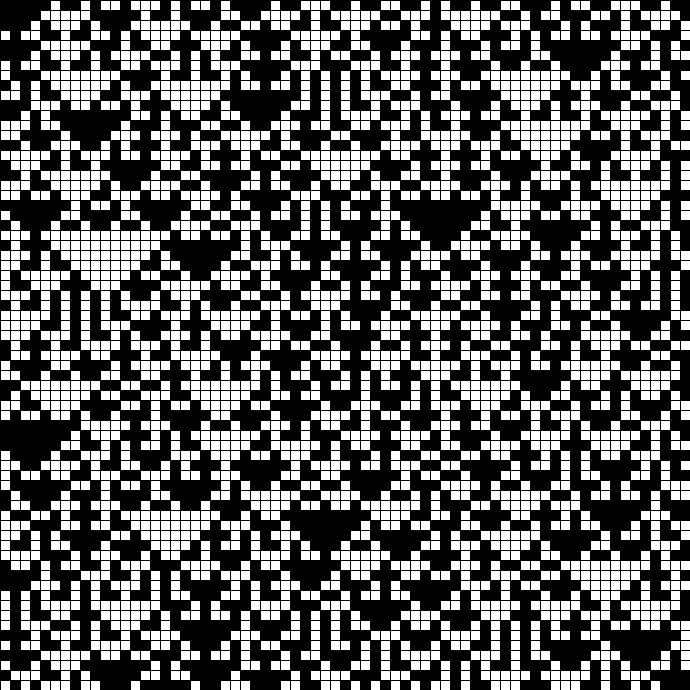
\includegraphics[width=0.33\textwidth]{figs/rule-150b.png}}\label{fig:st-eca150}}\quad
	\subfloat[]{\fbox{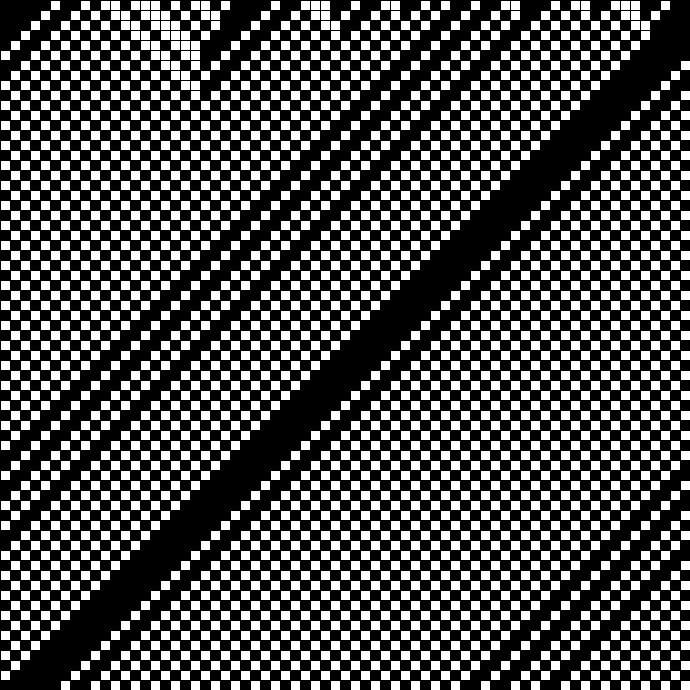
\includegraphics[width=0.33\textwidth]{figs/rule-184b.png}}\label{fig:st-eca184}}\\
	\subfloat[]{\fbox{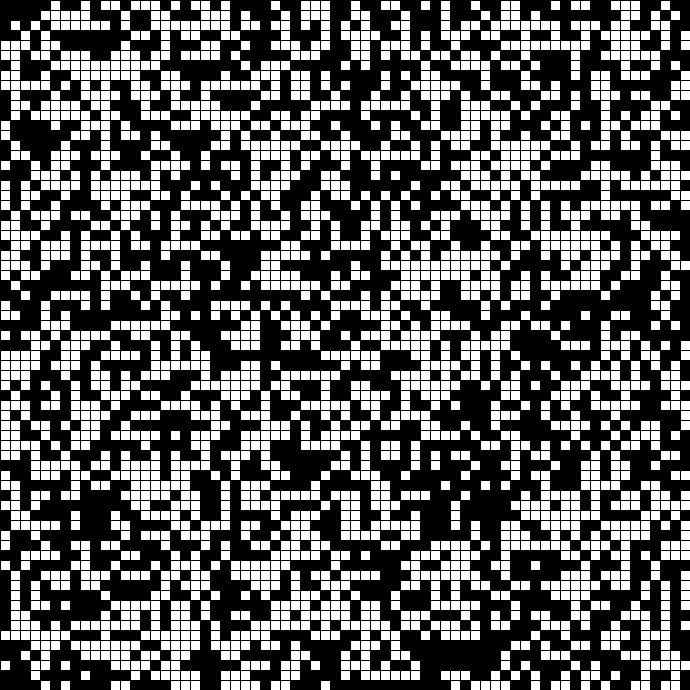
\includegraphics[width=0.33\textwidth]{figs/rule-150-gap.png}}\label{fig:ob-eca150}}\quad
	\subfloat[]{\fbox{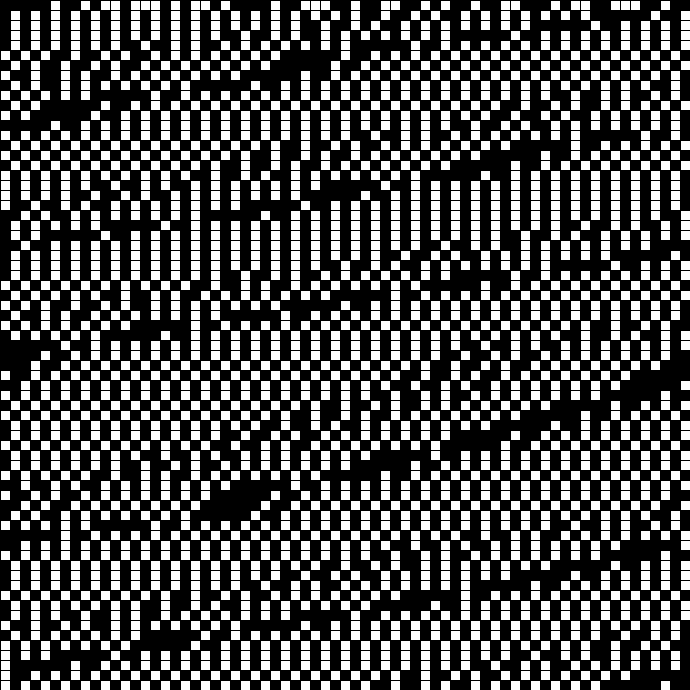
\includegraphics[width=0.33\textwidth]{figs/rule-184-gap.png}}\label{fig:ob-eca184}}
	\caption{Space-time diagrams of (\protect\subref*{fig:st-eca150}) ECA 150 and (\protect\subref*{fig:st-eca184}) ECA 184 containing 69 cells and 69 time stamps each, and the (\protect\subref*{fig:ob-eca150}), (\protect\subref*{fig:ob-eca184}) corresponding temporally incomplete observations with random time gaps of at most ten time steps.}\label{fig:space-time-example}
\end{figure*}

In both experiments, the GA quickly found a solution. In the case of experiment R1 it took 26 iterations, while 23 iterations were needed in experiment R2. In Fig.~\ref{fig:example-fitness} the maximum, average and minimum fitness of the population is shown over time for both experiments. Note that for the sake of readability the fitness values were normalized to the interval $[0,100]$.

\begin{figure}
	\centering
	\subfloat[]{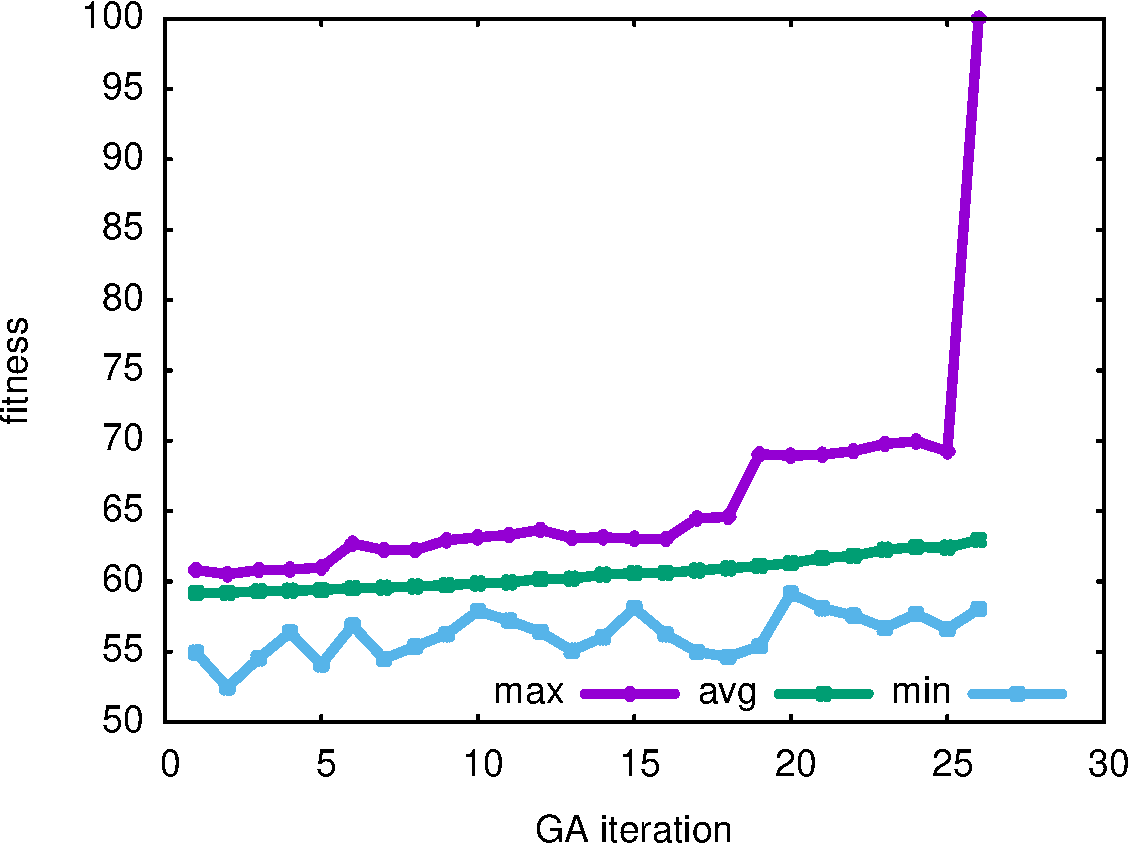
\includegraphics[width=0.45\textwidth]{figs/fit-150-crop.pdf}\label{fig:example-fit-r1}}\
	\subfloat[]{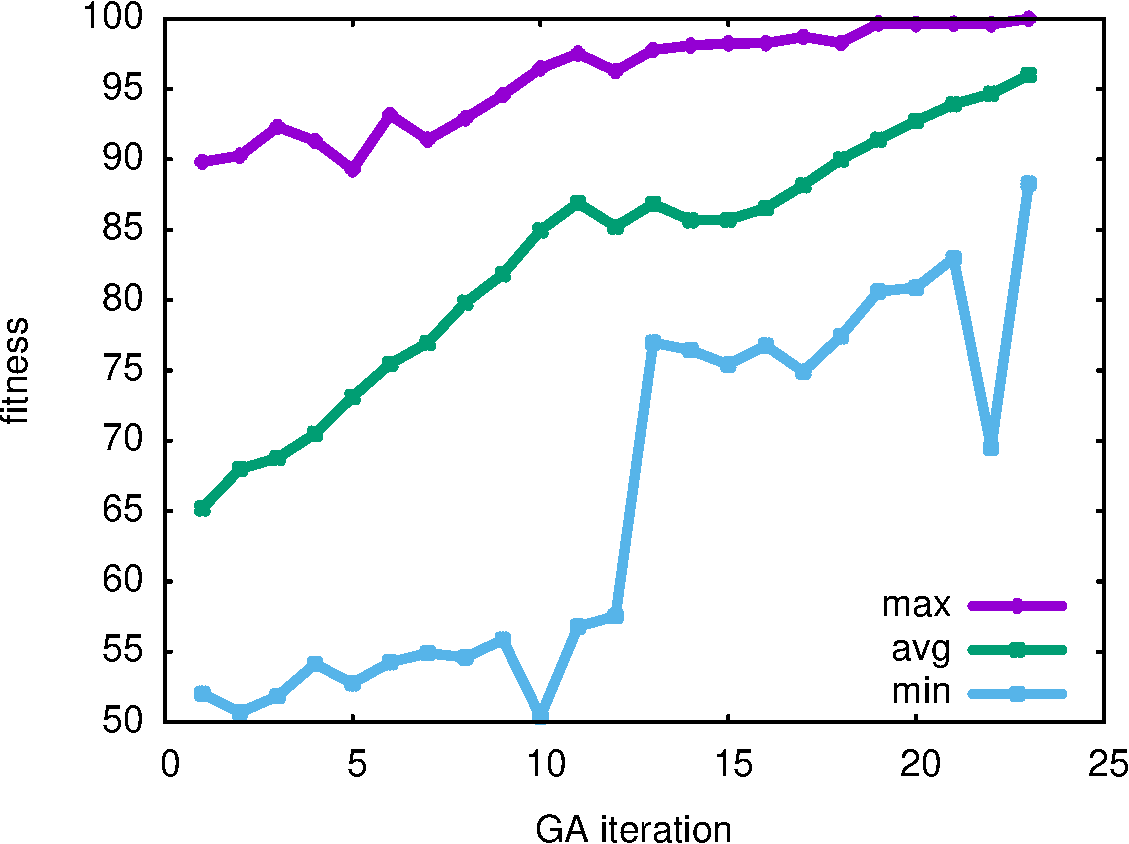
\includegraphics[width=0.45\textwidth]{figs/fit-184-crop.pdf}\label{fig:example-fit-r2}}
	\caption{The maximum, average and minimum fitness of the population versus the GA iteration in experiments (\protect\subref*{fig:example-fit-r1}) R1 and (\protect\subref*{fig:example-fit-r2}) R2.}\label{fig:example-fitness}
\end{figure}

Firstly, let us note that the plotted values correspond to the fitness approximation calculated over a subset of the observation set as described in Section~\ref{sec:fitness}. This explains why the maximum is not strictly increasing, though the algorithm uses an elite survival procedure.

Moreover, as can be seen in the plots, in both experiments the average fitness (almost) constantly increased as the populations evolved. In R1 the growth was stable but slow, while in the case of R2 we see a more rapid increase, especially during the first 10 iterations. In the case of R1, the final solution was found within one significant ``jump'' of the maximal fitness. This can be attributed to the fact that the behavior of CAs that are very close to the best solution is completely different from the one of ECA 150. In contrast, in R2 we see a rather gentle increase of the maximum fitness towards 100, which can be explained by the fact that there are many CAs resulting in checkerboard-like patterns similar to the ones evolved by ECA 184.

\begin{figure*}
	\centering
	\begin{tabular}{ccccc}
		\fbox{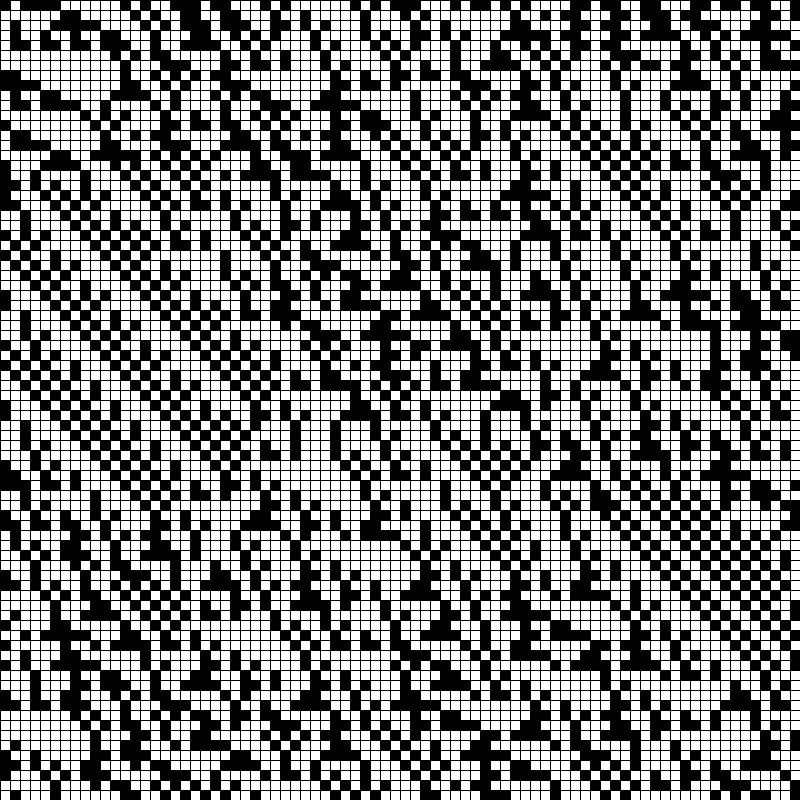
\includegraphics[width=0.17\textwidth]{figs/rule-150-best/rule-150-eval-1.png}}
		  &
		\fbox{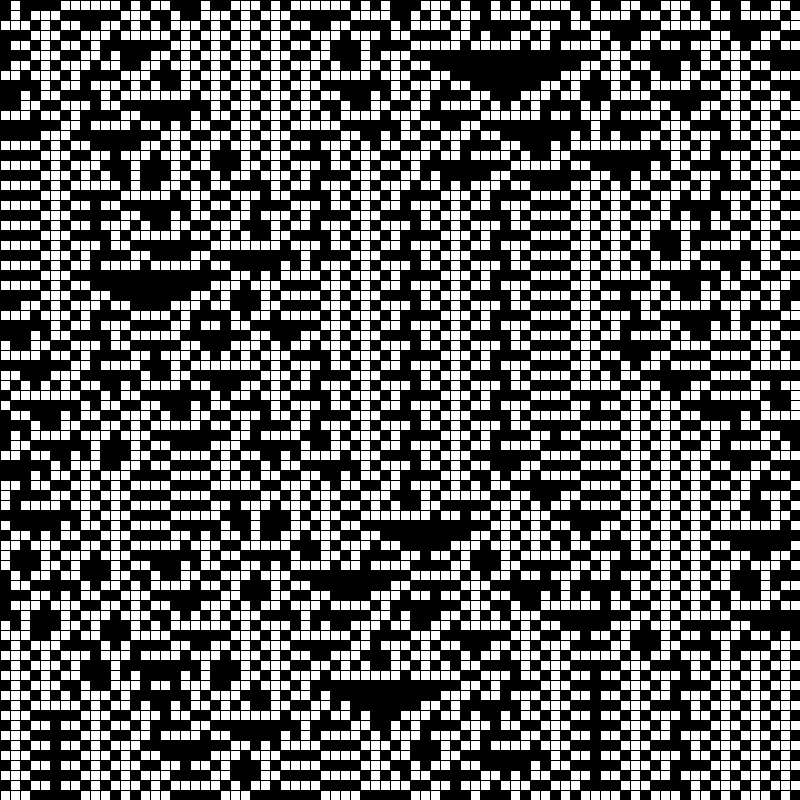
\includegraphics[width=0.17\textwidth]{figs/rule-150-best/rule-150-eval-2.png}}
		  &
		\fbox{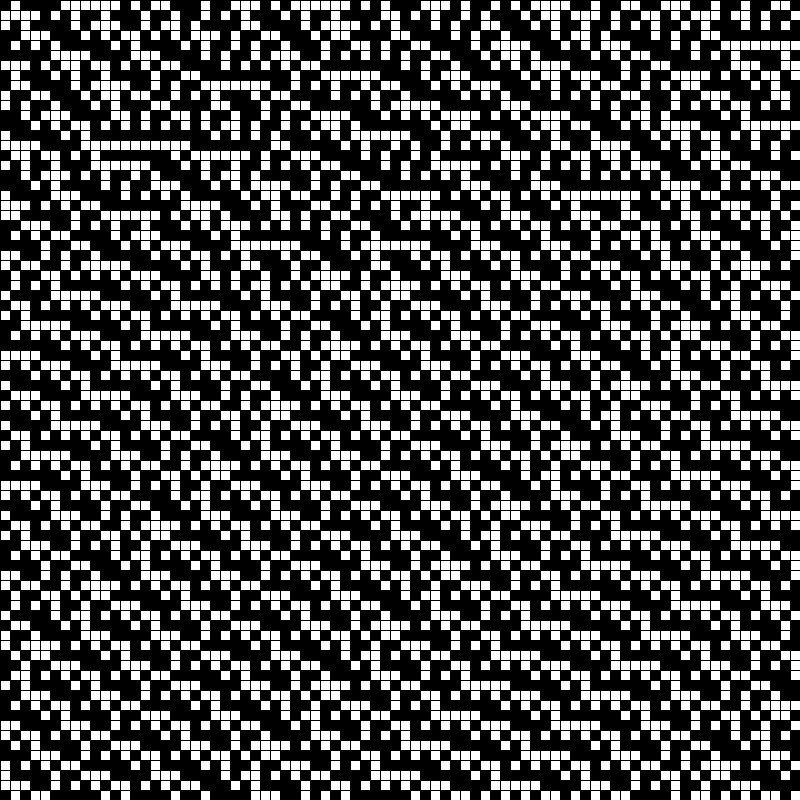
\includegraphics[width=0.17\textwidth]{figs/rule-150-best/rule-150-eval-3.png}}
		  &
		\fbox{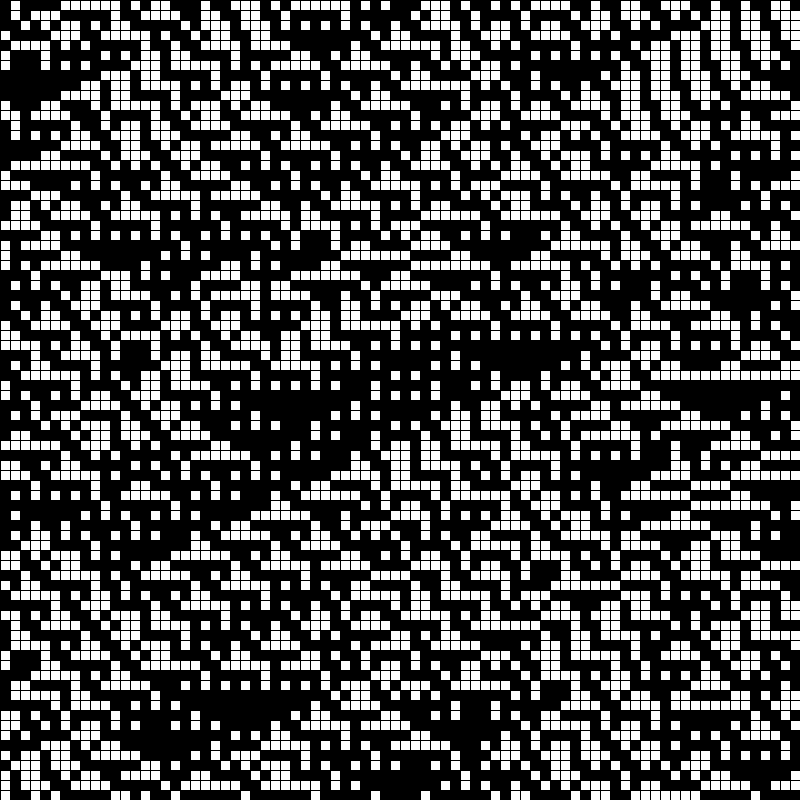
\includegraphics[width=0.17\textwidth]{figs/rule-150-best/rule-150-eval-4.png}}
		  &
		\fbox{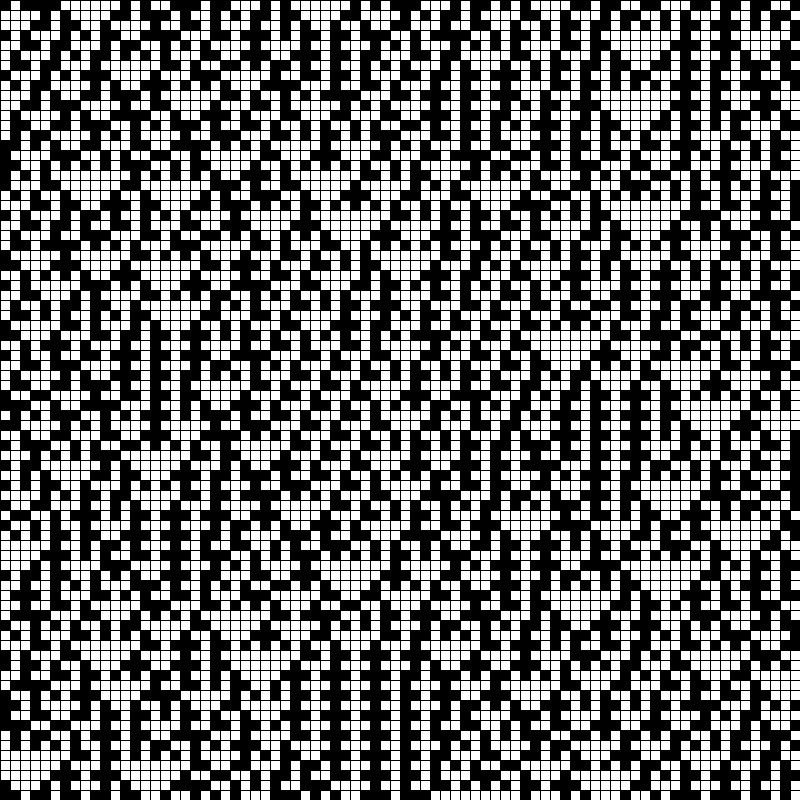
\includegraphics[width=0.17\textwidth]{figs/rule-150-best/rule-150-eval-5.png}}
		\\
		1 & 3  & 4  & 5  & 6                                                              \\
		\fbox{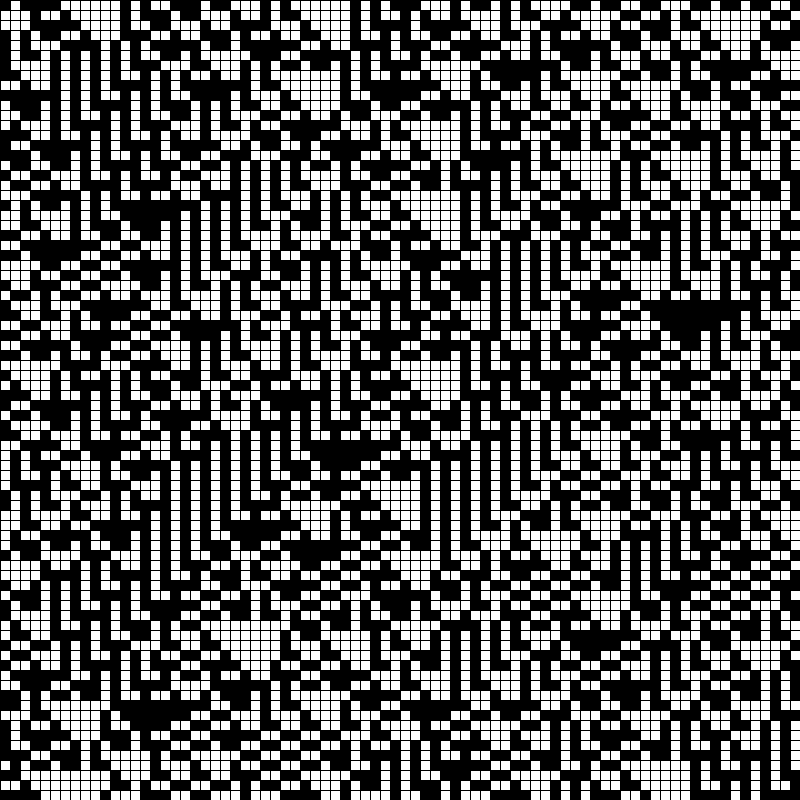
\includegraphics[width=0.17\textwidth]{figs/rule-150-best/rule-150-eval-6.png}}
		  &
		\fbox{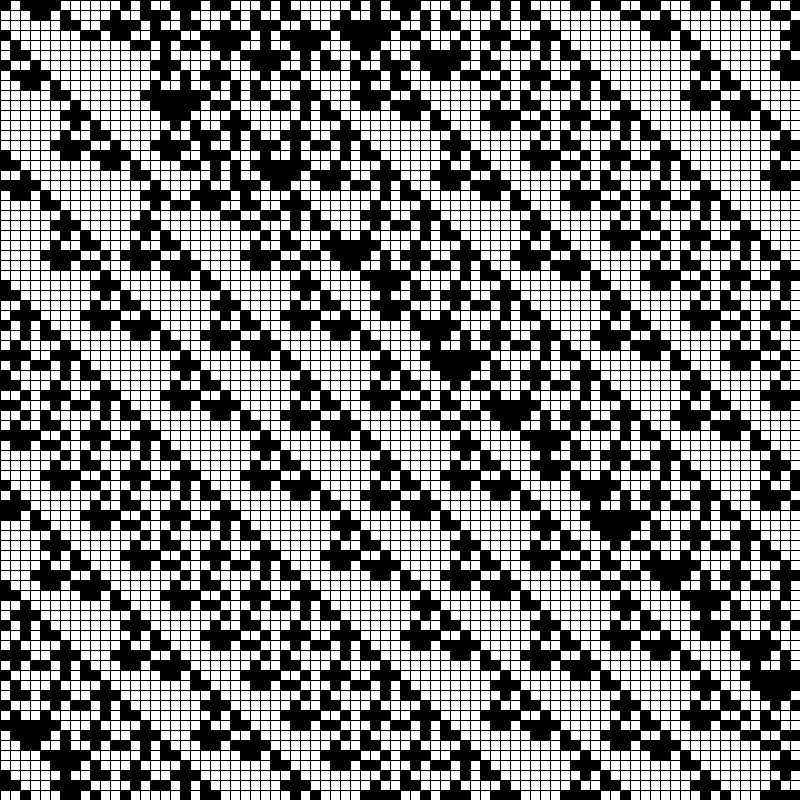
\includegraphics[width=0.17\textwidth]{figs/rule-150-best/rule-150-eval-10.png}}
		  &
		\fbox{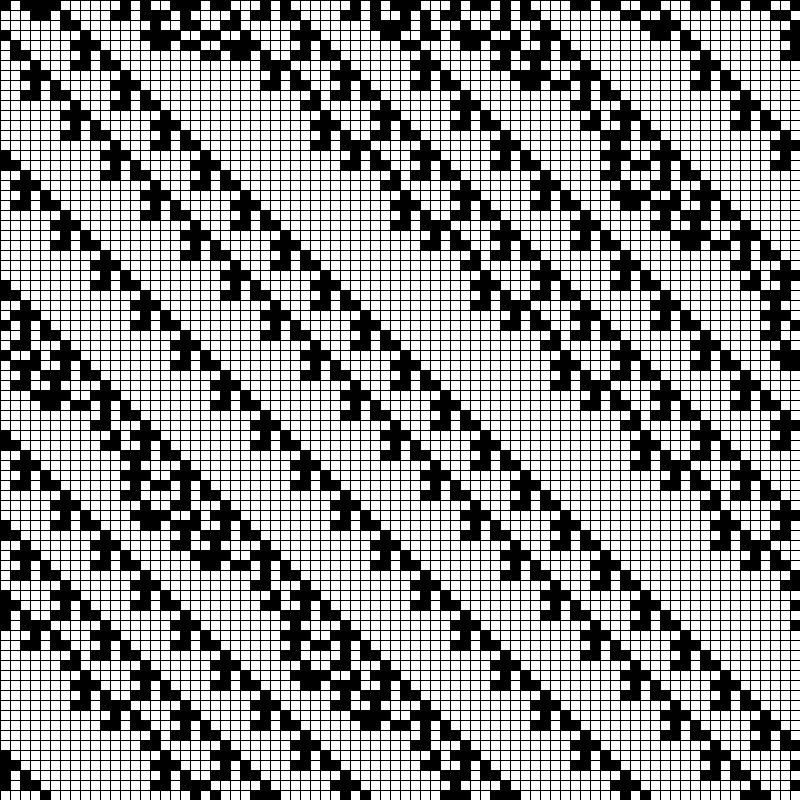
\includegraphics[width=0.17\textwidth]{figs/rule-150-best/rule-150-eval-12.png}}
		  &
		\fbox{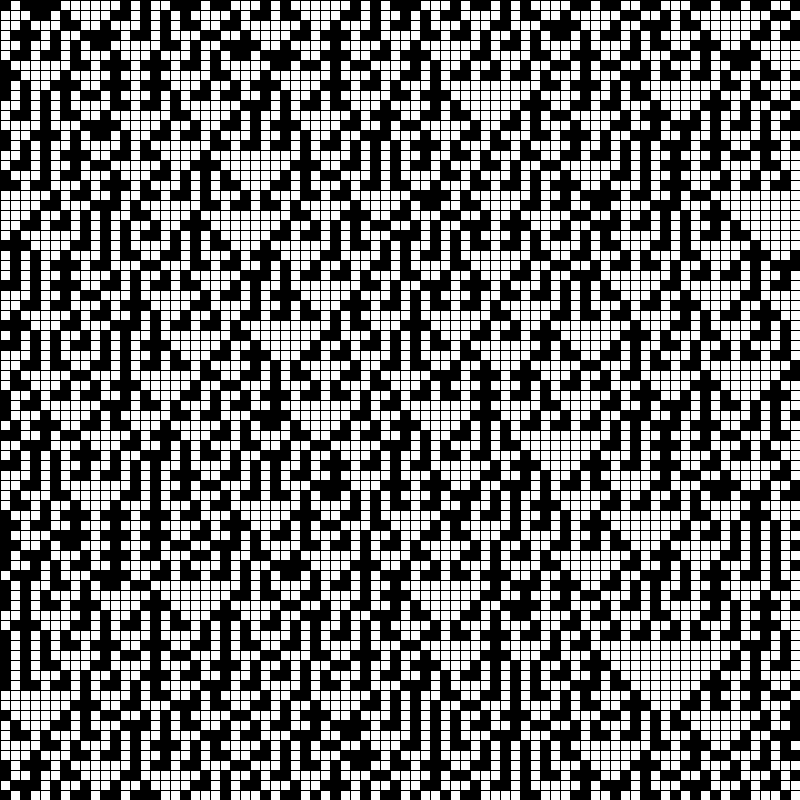
\includegraphics[width=0.17\textwidth]{figs/rule-150-best/rule-150-eval-15.png}}
		  &
		\fbox{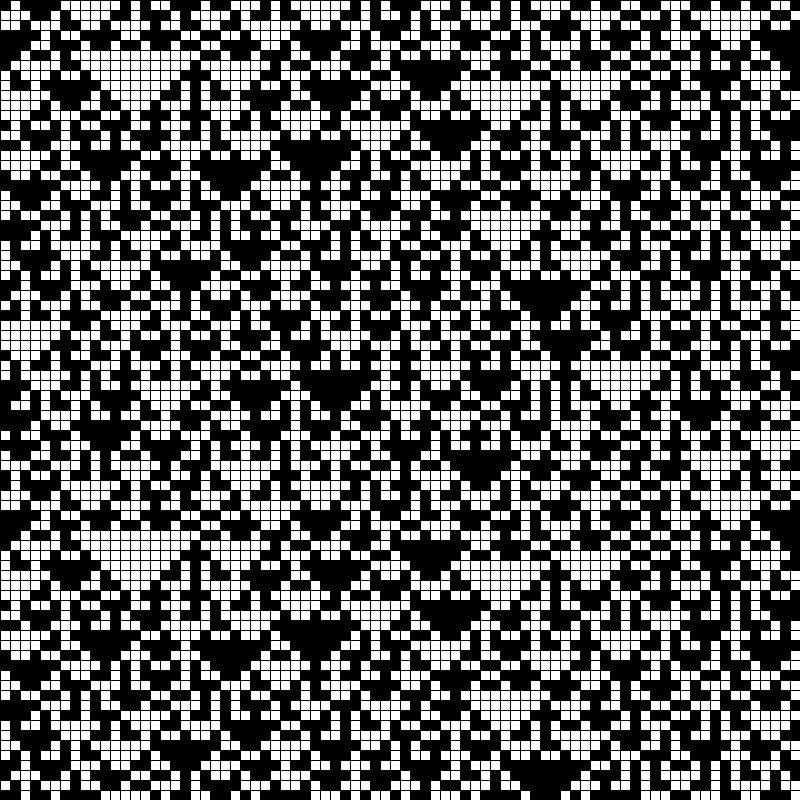
\includegraphics[width=0.17\textwidth]{figs/rule-150-best/rule-150-eval-16.png}} \\
		9 & 17 & 19 & 24 & 26                                                             \\
	\end{tabular}
	\caption{Current best individuals visualized with their space-time diagram and the corresponding GA iteration number, in R1.}\label{fig:best-150}
\end{figure*}

\begin{figure*}
	\centering
	\begin{tabular}{ccccc}
		\fbox{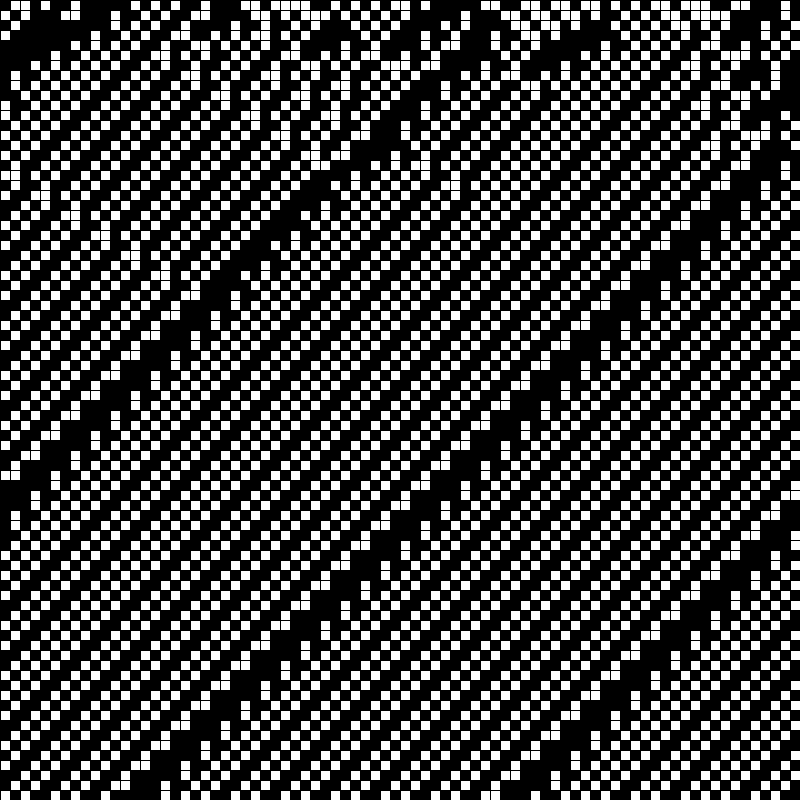
\includegraphics[width=0.17\textwidth]{figs/rule-184-best/rule-184-eval-1.png}}
		   &
		\fbox{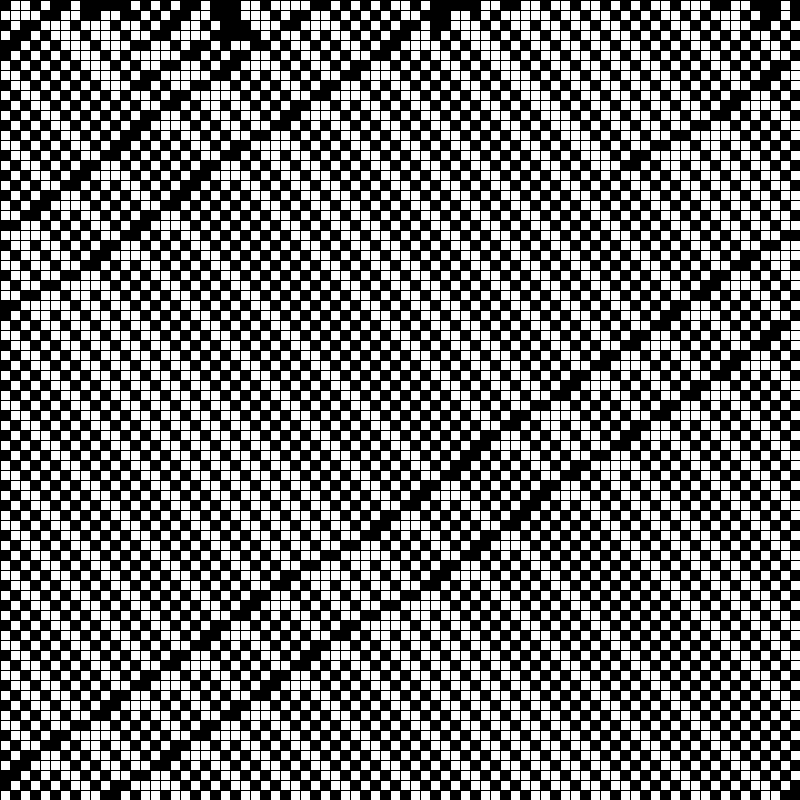
\includegraphics[width=0.17\textwidth]{figs/rule-184-best/rule-184-eval-2.png}}
		   &
		\fbox{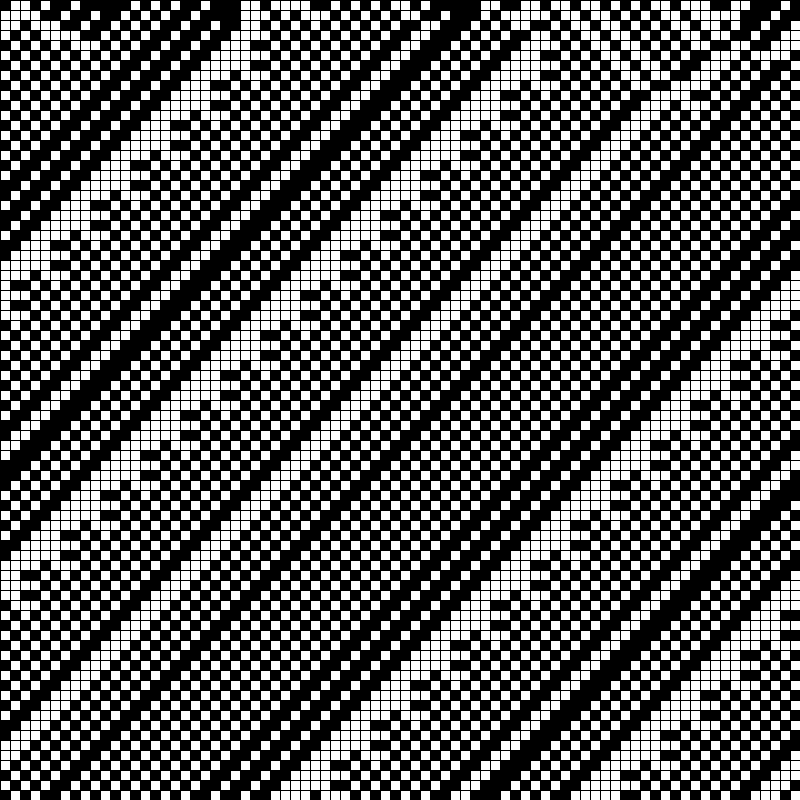
\includegraphics[width=0.17\textwidth]{figs/rule-184-best/rule-184-eval-3.png}}
		   &
		\fbox{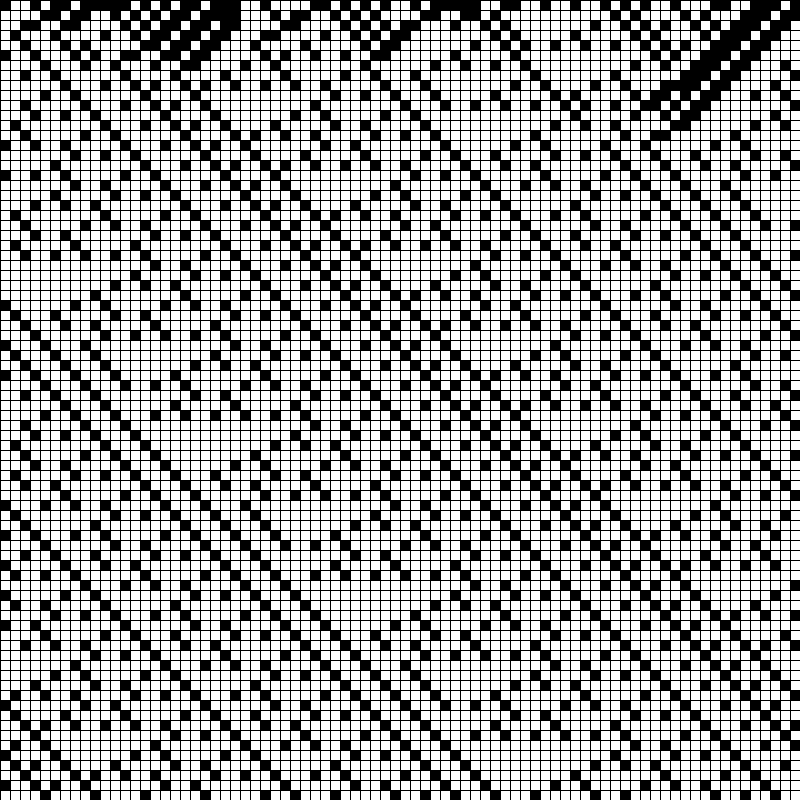
\includegraphics[width=0.17\textwidth]{figs/rule-184-best/rule-184-eval-4.png}}
		   &
		\fbox{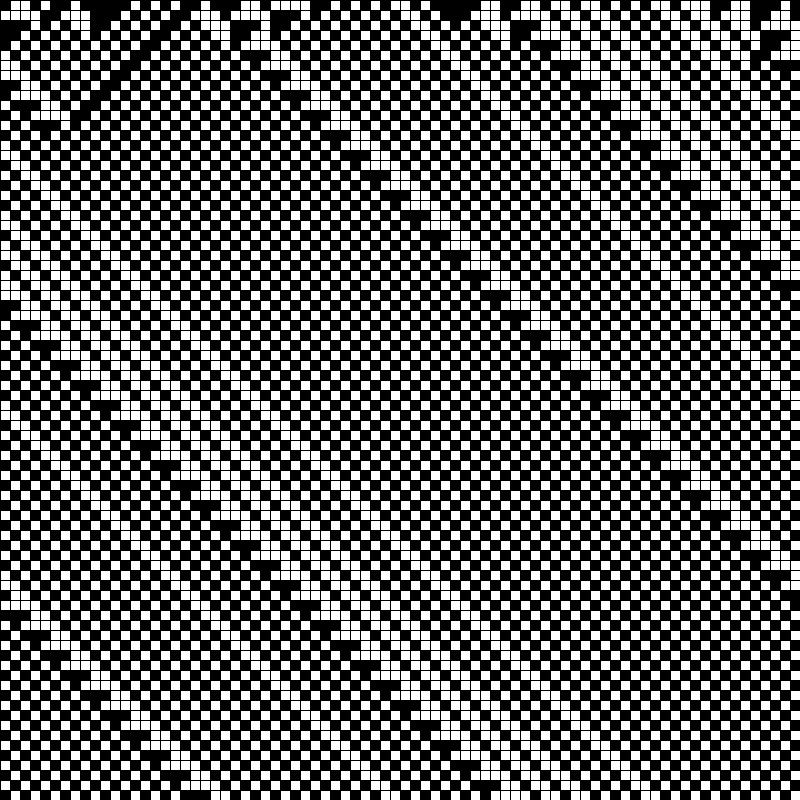
\includegraphics[width=0.17\textwidth]{figs/rule-184-best/rule-184-eval-5.png}}
		\\
		1  & 3  & 6  & 9  & 10 \\
		\fbox{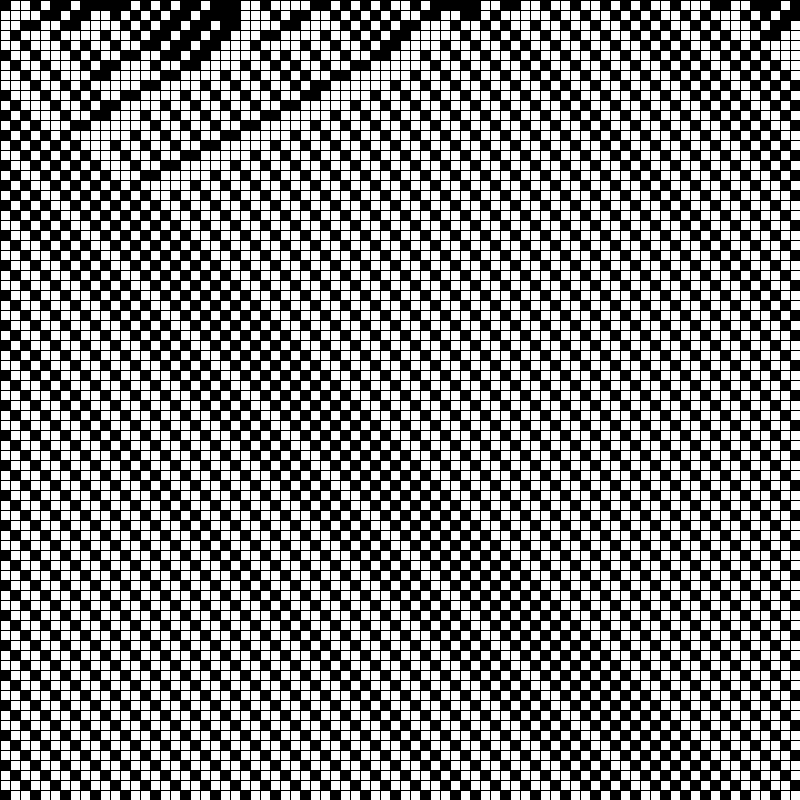
\includegraphics[width=0.17\textwidth]{figs/rule-184-best/rule-184-eval-6.png}}
		   &
		\fbox{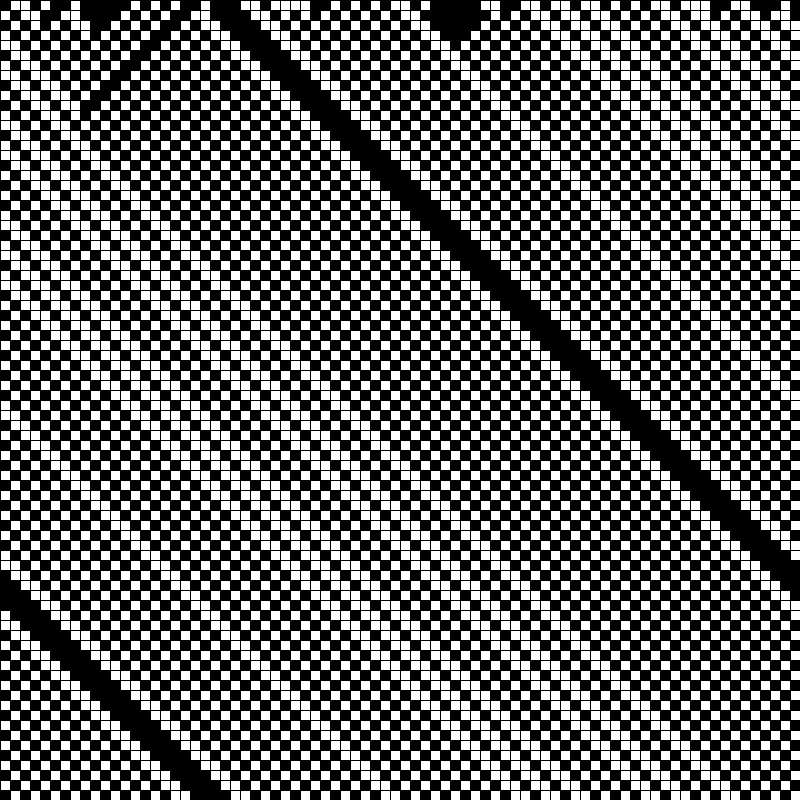
\includegraphics[width=0.17\textwidth]{figs/rule-184-best/rule-184-eval-7.png}}
		   &
		\fbox{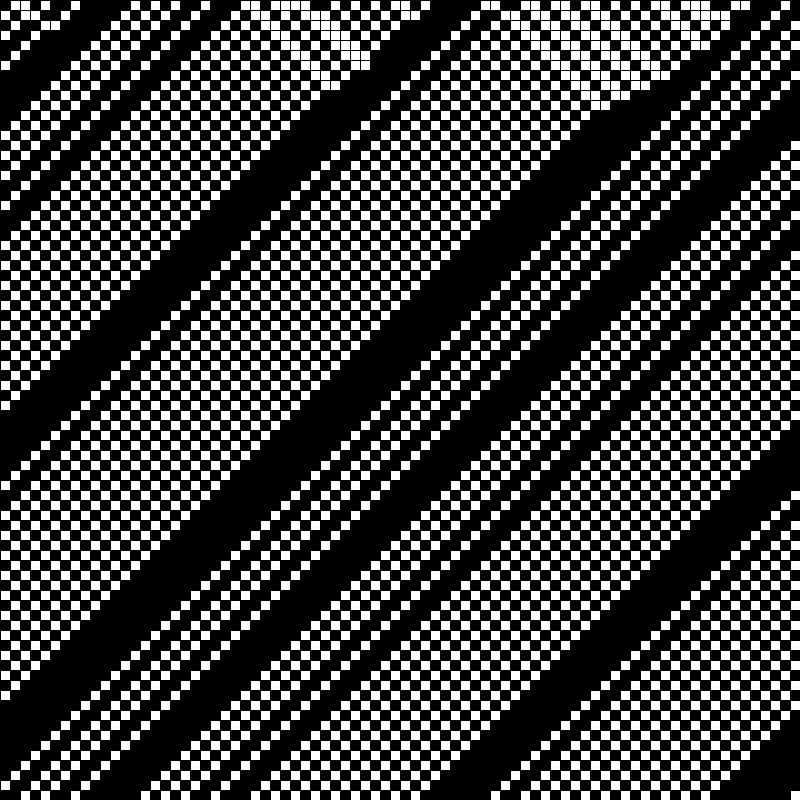
\includegraphics[width=0.17\textwidth]{figs/rule-184-best/rule-184-eval-8.png}}
		   &
		\fbox{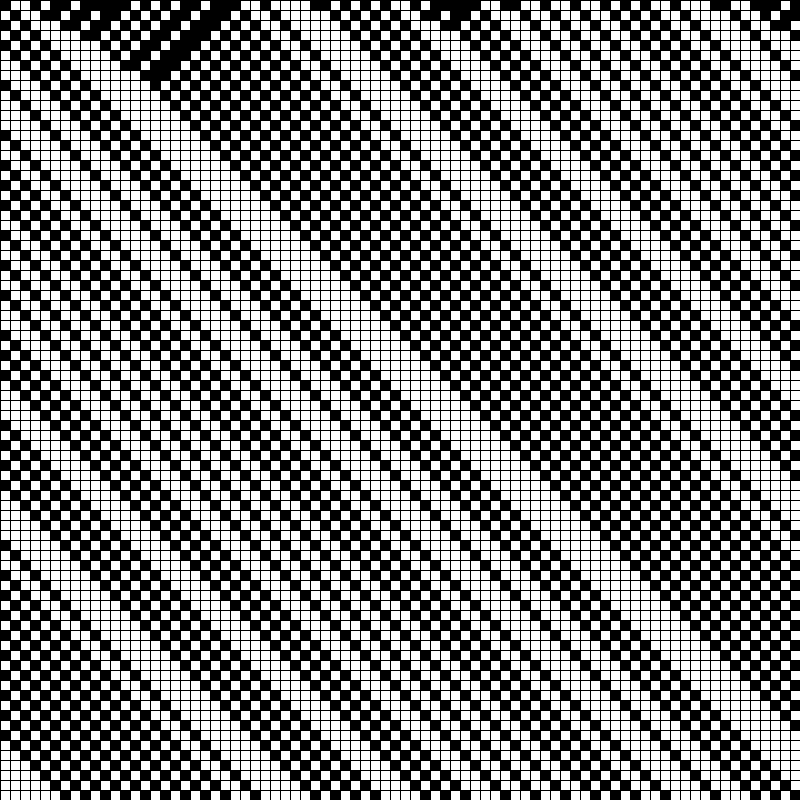
\includegraphics[width=0.17\textwidth]{figs/rule-184-best/rule-184-eval-9.png}}
		   &
		\fbox{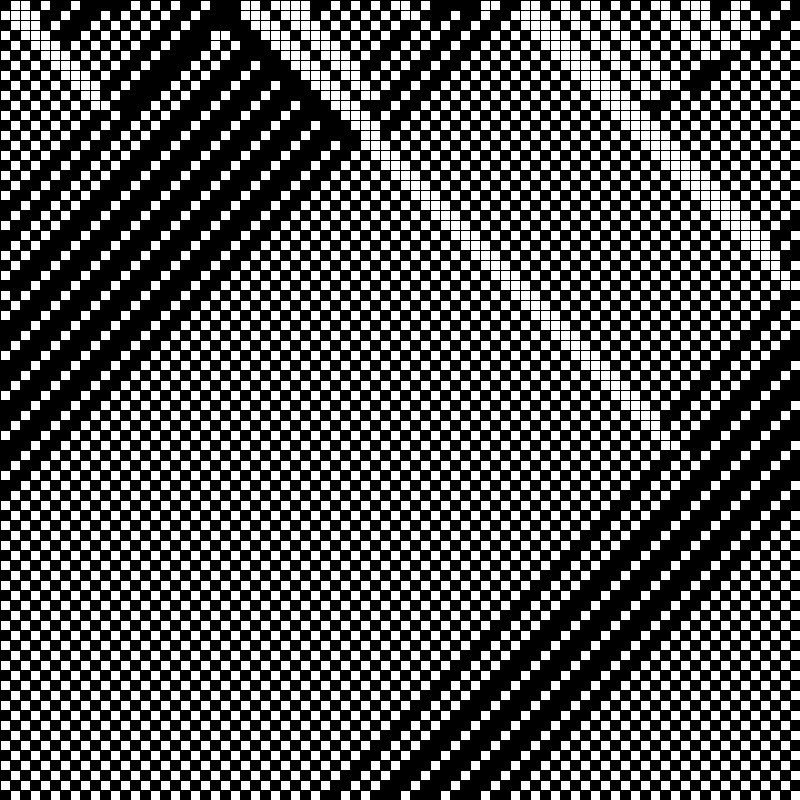
\includegraphics[width=0.17\textwidth]{figs/rule-184-best/rule-184-eval-11.png}}
		\\
		11 & 13 & 14 & 15 & 17 \\
		\fbox{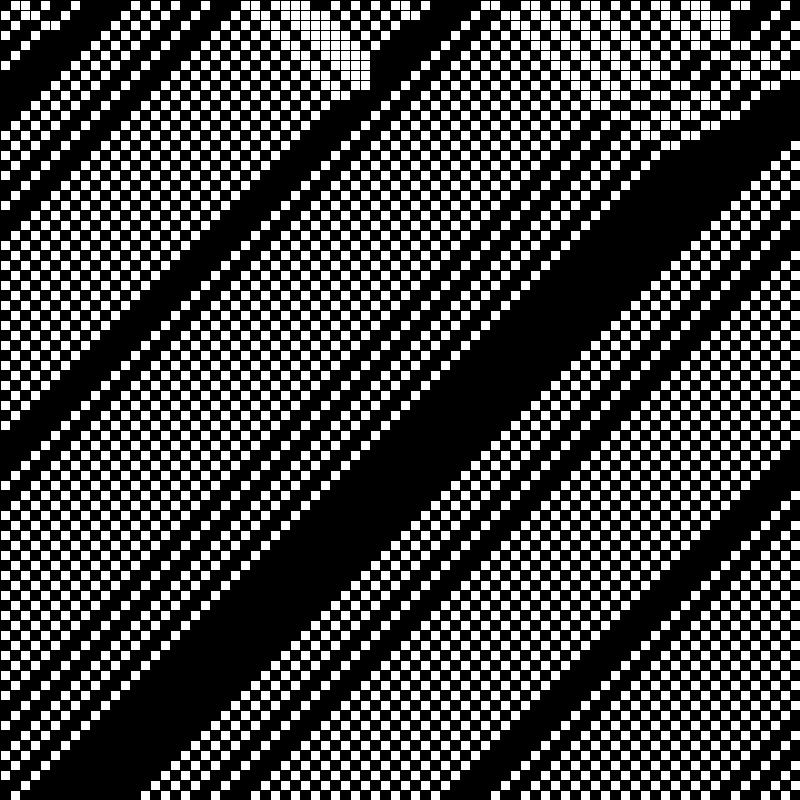
\includegraphics[width=0.17\textwidth]{figs/rule-184-best/rule-184-eval-12.png}}
		   &
		\fbox{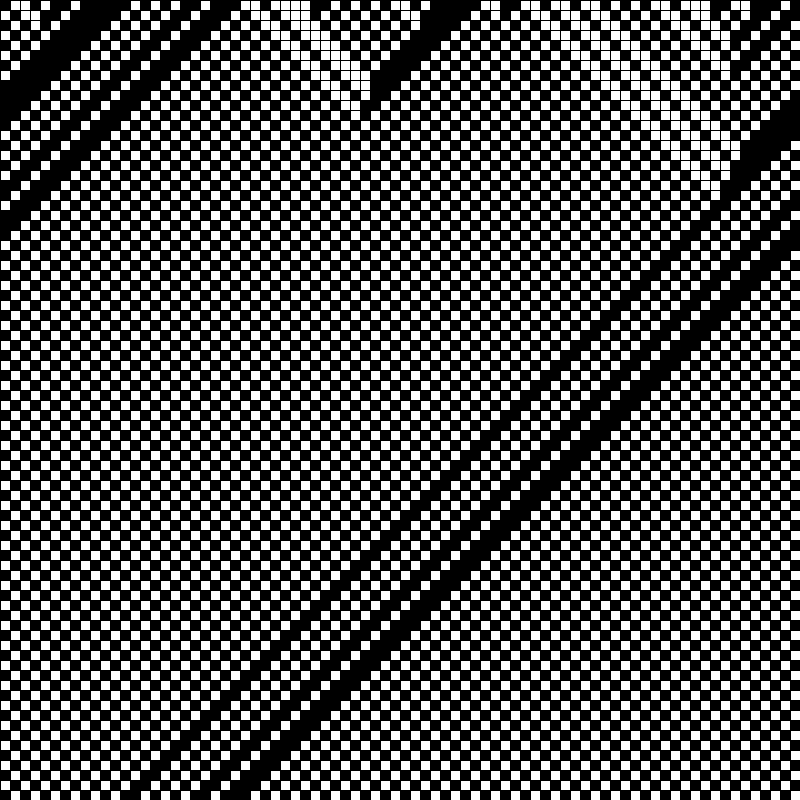
\includegraphics[width=0.17\textwidth]{figs/rule-184-best/rule-184-eval-13.png}}
		   &
		   &
		   &
		\\
		19 & 23 &    &    &
	\end{tabular}
	\caption{Current best individuals visualized with their space-time diagram and the corresponding GA iteration number, in R2.}\label{fig:best-184}
\end{figure*}

In Fig.~\ref{fig:best-150} we see the space-time diagram of some CAs that  were discovered by the GA during the evolution as ``current best'' candidates for R1, while Fig.~\ref{fig:best-184} displays these for R2.

Interestingly, in both experiments, relatively early in the evolution the GA was able to concentrate on some of the crucial patterns in the space-time diagrams of the unknown ECAs. In R1, after 6 iterations, the best individuals already replicated the triangular pattern of ECA 150, even though it is very hard to notice such a pattern in the observations available for the GA (see Fig.~\ref{fig:ob-eca150}). Similarly, in R2, the linear pattern emerged very quickly, yet deciding on the slope of the lines turned out to be a bit more challenging.

\section{Experimental results}\label{sec:experiments}%
\subsection{Introduction}
In this section the results of a series of computational experiments are presented. The main goal of these experiments was to evaluate the effectiveness of the identification algorithm in specific circumstances, where the observation set is generated by a selected CA. The goal of the GA was to uncover this CA from observations. Five experiments were performed and in each of them a broad class of CAs and corresponding observation sets were considered. In Experiment~1 we evaluated the performance of the GA on spatially complete observation sets originating from the entire class of ECAs, considered as a subset of $\mathcal{A}_2$, \emph{i.e.}\ CAs with radius 2. By only considering ECAs, we were able to examine a class of well-known CAs. Yet, considering such a specific subset of $\mathcal{A}_2$ may have had a strong impact on the results. To verify whether this was the case, Experiment~2 was conducted, where we evaluated the performance of the GA on observations originating from a randomly selected set of 350 CAs defined by local rules with radius 2 (but not ECAs). In Experiments 2 and 4, the lengths of the time gaps were random. To verify whether this uniform randomness influences the obtained results, we studied other types of time gaps (constant vs.\ only odd vs.\ only even) in Experiment 3. In Experiment~4 we additionally considered spatially incomplete observations. Finally, Experiment~5 covers the aspect of radius detection, \emph{i.e.}\ the ability of the GA to uncover the correct radius of the underlying CA (which is not known upfront in many practical cases). Three cases were studied here, namely CAs with radius 2, 3 and 4.

Due to the large number of cases in the experiments described in this section, the GA has been implemented using highly optimized code written in C and compiled by the Intel C compiler, utilizing OpenMP for concurrent fitness calculations. The specific executions of the GA were run on a large computing cluster, where each execution was bound to a specific node (no inter-node communication was needed). Each of the cluster's nodes had a 24-core Xeon E5-2670 CPU and 128 GB of RAM. The source code of this GA implementation along with the build and execution scripts and technical documentation is available on: \href{https://github.com/houp/identify}{github.com/houp/identify}.

\subsection{Experiment 1: Identification of ECAs in case of spatial completeness}
In this experiment, the observation set $\mathcal{I}$ consists of spatially complete observations only, \emph{i.e.}\ for every $I\in\mathcal{I}$, it holds that $I\in\{0,1\}^{N_I\times M_I}$. In addition, we assume that the number of rows is equal to the number columns in all observations ($N_I = M_I = S > 0$).

The goal of the experiment is to measure the efficiency of the identification algorithm. More specifically, we are interested in the number of iterations needed in order to evolve to a solution. We assess the performance of the algorithm using observation sets generated by ECA rules. Let $\mathcal{I}_{A}$ denote the observation set obtained by observing the behavior of an ECA $A$. It is assumed that for each $A$, the number of observations is the same, \emph{i.e.}\ $\abs{\mathcal{I}_A} = K$, for $K>0$, and that the observations of different ECAs are evolved from the same set of random initial conditions. Observation set $\mathcal{I}_A$ contains observations with random time gaps bounded by $\Gamma>0$, which are chosen for every row independently.

The values of the design parameters used in this experiment are the same as in Table~\ref{tab:example-params} with the exception of: $P=32$, $P_E=8$, $\alpha=0.0.25$, $R=100$. Due to the stochastic nature of the GA, the experiment is repeated $\Omega=50$ times for each ECA.

The performance of the GA is quantified for each $A$ in terms of the average ($\avg_A$), minimum ($\min_A$) and maximum ($\max_A$) number of GA iterations needed to find the solution. Across all ECAs, the average of the minimum, average and maximum number of GA iterations was 46, 270 and 1018, respectively.

These results may serve as a reference when interpreting the statistics broken down for specific behavioral classes (Tables~\ref{tab:exp1-wolf} and~\ref{tab:exp1-lyap}). In Table~\ref{tab:exp1-wolf} the grouping is done according to Wolfram's classification scheme~\cite{RevModPhys.55.601}, while the values of the normalized maximum Lyapunov exponent (nMLE)~\cite{Wolfram:84,Sher:92,citeulike:9312129} are used in Table~\ref{tab:exp1-lyap}. These tables show that the effort needed for identification is significantly lower than the overall average for ECAs belonging to the least complex classes (Wolfram Class~I and $\textrm{nMLE}=-\infty$). Additionally, the most complex classes require the highest average number of iterations, which shows that there is a connection between the complexity of a CA's dynamical nature and the performance of the identification algorithm. This connection is further confirmed by the results of a two-sided Mann--Whitney $U$ test for $\avg_A$ grouped according to Wolfram's classes (Table~\ref{tab:stat1-wolf}) and the nMLE  (Table~\ref{tab:stat1-lyap}). The p-values confirm that the difference in performance of the GA for the different Wolfram classes and for the considered (intervals of) nMLE values is statistically significant.
\begin{table}[ht]
	\centering
	\caption{Experiment 1: The performance of the GA expressed in terms of the average of the minimum, average and maximum number of iterations per behavioral class according to Wolfram's classification scheme \protect\subref*{tab:exp1-wolf} and the nMLE~\protect\subref*{tab:exp1-lyap}.}
	\subfloat[]{\label{tab:exp1-wolf}
		\begin{tabular}{c|c|c|c}
			{\bf class} & {\bf avg($\min_A$)} & {\bf avg($\avg_A$)} & {\bf avg($\max_A$)} \\ \hline
			{\bf I}     & 38                  & 207                 & 666                 \\
			{\bf II}    & 47                  & 244                 & 915                 \\
			{\bf III}   & 40                  & 296                 & 1264                \\
			{\bf IV}    & 57                  & 690                 & 2650                \\
		\end{tabular}}\quad
	\subfloat[]{\label{tab:exp1-lyap}
		\centering
		\begin{tabular}{c|c|c|c}
			{\bf nMLE}     & {\bf avg($\min_A$)} & {\bf avg($\avg_A$)} & {\bf avg($\max_A$)} \\ \hline
			$\bm{-\infty}$ & 44                  & 257                 & 934                 \\
			$\bm0$         & 38                  & 176                 & 665                 \\
			$\bm{>0}$      & 49                  & 308                 & 1187                \\
		\end{tabular}}
\end{table}

\begin{table}[ht]
	\centering
	\caption{Experiment 1: Results of the two-sided Mann--Whitney $U$ test of $\avg_A$ grouped according to Wolfram's classification scheme~\protect\subref*{tab:stat1-wolf} and the nMLE~\protect\subref*{tab:stat1-lyap}.}\label{tab:mannwhitney}
	\subfloat[]{\label{tab:stat1-wolf}
		\begin{tabular}{c|c|c}
			case                    & $U$-statistic & p-value      \\ \hline
			Class I vs.\ Class II   & 1858          & 1.227561e-01 \\
			Class I vs.\ Class III  & 167           & 5.016731e-03 \\
			Class I vs.\ Class IV   & 63            & 1.565208e-03 \\ \hline
			Class II vs.\ Class III & 1606.5        & 3.226133e-03 \\
			Class II vs.\ Class IV  & 564           & 2.946143e-04 \\ \hline
			Class III vs.\ Class IV & 123           & 9.714852e-02
		\end{tabular}}\quad
	\subfloat[]{\label{tab:stat1-lyap}
		\begin{tabular}{c|c|c}
			case                                               & $U$-statistic & p-value      \\ \hline
			$\textrm{nMLE} = -\infty$ vs.\ $\textrm{nMLE} = 0$ & 2095          & 1.859012e-02 \\
			$\textrm{nMLE} = -\infty$ vs.\ $\textrm{nMLE} > 0$ & 4671          & 3.475995e-01 \\
			$\textrm{nMLE} = 0$ vs.\ $\textrm{nMLE} > 0$       & 1848.5        & 5.748794e-05
		\end{tabular}}
\end{table}

In Table~\ref{tab:exp1-rest} we present the nMLE and GA statistics of the five ECAs that were the easiest to identify (Table~\ref{tab:exp1-res}) and the five ECAs that were the hardest to identify (Table~\ref{tab:exp1-res2}) according to the values of $\avg_A$. Not surprisingly, among the easiest to identify, we find ECAs 0 and 255, which correspond to the two simplest local rules mapping any neighborhood configuration to the same value. Interestingly, all of the ECAs that were hard to identify have similar relatively high nMLE values. Summing up, the identification algorithm turns out to be effective in all of the cases considered, although the effort of finding a solution differs greatly, depending on the ECA.

\begin{table}[ht]
	\centering
	\caption{ECAs requiring the smallest \protect\subref*{tab:exp1-res} and the largest \protect\subref*{tab:exp1-res2} number of iterations of the GA in Experiment 1.}\label{tab:exp1-rest}
	\subfloat[]{
		\begin{tabular}{c|c|c|c|c}
			{\bf ECA} & {\bf nMLE} & $\textbf{min}_A$ & ${\textbf{avg}_A}$ & ${\textbf{max}_A}$ \\ \hline
			{\bf 255} & $-\infty$  & 1                & 3                  & 9                  \\
			{\bf 0}   & $-\infty$  & 4                & 30                 & 183                \\
			{\bf 221} & $-\infty$  & 25               & 47                 & 86                 \\
			{\bf 207} & $0$        & 25               & 55                 & 156                \\
			{\bf 246} & $0$        & 27               & 57                 & 112
		\end{tabular}\label{tab:exp1-res}}\
	\subfloat[]{
		\begin{tabular}{c|c|c|c|c}
			{\bf ECA} & {\bf nMLE} & $\textbf{min}_A$ & ${\textbf{avg}_A}$ & ${\textbf{max}_A}$ \\ \hline
			{\bf 137} & $0.6577$   & 48               & 1679               & 8270               \\
			{\bf 193} & $0.6561$   & 52               & 1625               & 6221               \\
			{\bf 110} & $0.6574$   & 49               & 1348               & 4269               \\
			{\bf 25}  & $0.5168$   & 43               & 1262               & 5690               \\
			{\bf 124} & $0.6567$   & 59               & 1231               & 4431
		\end{tabular}\label{tab:exp1-res2}
	}
\end{table}

\subsection{Experiment 2: Performance on the class $\mathcal{A}_2$}

Experiment 1 concerned ECAs only, considering them as a subclass of $\mathcal{A}_2$, by setting $r_\ast = 2$ in the GA, so that a measurable effort was needed to find a solution. As a natural continuation of Experiment 1, we repeated the experiment, but instead of using 256 ECAs to generate initial observation sets, we used 350 randomly selected CAs defined by a local rule with radius two, \emph{i.e.}\ CAs belonging to the class $\mathcal{A}_2$. The remaining parameters and experimental setup were the same as in Experiment 1. The goal of this experiment was to verify whether the results of Experiment 1~were affected by the nature of ECAs, which form a very specific subclass of $\mathcal{A}_2$.

The average of the minimum, average and maximum number of GA iterations required to find a solution in this experiment was, respectively:
\[\avg(\min{}_A) = 57,\ \avg(\avg_A) = 617,\ \avg(\max{}_A) = 3040\,.\]

These results clearly suggest that, on average, ECAs as a subclass of $\mathcal{A}_2$ were easier to identify compared to other CAs from the class $\mathcal{A}_2$, which may be attributed to the fact that many of the ECAs result in a relatively simple dynamical behavior. On the other hand, although the averages are slightly higher, the order of magnitude is not changed. We believe that these results show that the approach of analyzing ECAs as a subclass of $\mathcal{A}_2$ in Experiment 1 was fully justified. More interestingly, the results presented above are very close to the results for ECAs belonging to class IV of Wolfram's classification scheme (Table~\ref{tab:exp1-wolf}), suggesting that identification is likely to be more complex when identifying classes of CAs with higher radius.

\subsection{Experiment 3: Identification of ECAs with constant time gaps}
While the time gaps had a random length in Experiment 1, they are kept constant in this experiment. Random time gaps correspond to a lack of temporal synchronization between the observed system and the observations, while constant time gaps represent a simple form of synchronization of the clocks. Thus, the goal of this experiment is to verify whether such a synchronization makes it easier to solve the identification problem.

Each observation $I$ used in this experiment is constructed by randomly selecting one number $t_I \in \{1,\dotsc,\Gamma-1\}$ and taking every $t_I$-th row of the original space-time diagram, thus in between every two time stamps of a given observation $I$ exactly $t_I$ time stamps are missing. Neither the numbers $t_I$ nor the fact that the time gaps are equal are known by the GA. We consider three cases: 1) even $t_I$  (Table~\ref{tab:exp3a}); 2) odd $t_I$ (Table~\ref{tab:exp3b}); 3) arbitrary $t_I$ (Table~\ref{tab:exp3c}). The overall performance of the algorithm across all ECAs and these three cases are presented in Table~\ref{tab:exp3}.
\begin{table}[ht]
	\centering
	\caption{Experiment 3: The performance of the GA expressed in terms of the average of the minimum, average and maximum number of iterations in the case of: 1.\ even, 2.\ odd and 3.\ arbitrary time gaps.}\label{tab:exp3}
	\begin{tabular}{r|l|c|c|c}
		{\bf case} & {\bf description}   & {\bf avg($\min_A$)} & {\bf avg($\avg_A$)} & {\bf avg($\max_A$)} \\ \hline
		{\bf 1}    & even time gaps      & 35                  & 158                 & 783                 \\
		{\bf 2}    & odd time gaps       & 1603                & 7074                & 16306               \\
		{\bf 3}    & arbitrary time gaps & 830                 & 4437                & 13152
	\end{tabular}
\end{table}

As can be inferred from these tables, the performance of the GA differs greatly from that in Experiment 1. Especially in the case of odd $t_I$, the performance is significantly lower. Moreover, in this case, for ECAs 105 and 150 (which are dynamically equivalent) the algorithm is not able to find a solution in fewer than $G=9\times 10^5$ iterations. A similar situation occurs in the case of arbitrary $t_I$ (Table~\ref{tab:exp3c}), where the effect of odd time gaps, which are present in about half of the cases, played an important role.

The reason for the unidentifiability of ECAs 105 and 150 lies in the specific properties of binary CAs. Let $A_{105}$ and $A_{150}$ be the corresponding global rules of the ECAs in question. It is relatively easy to check that for any configuration $X$ it holds that $A_{105}(X) \neq A_{150}(X)$ and $A_{105}(A_{105}(X))~=~A_{150}(A_{150}(X))$. In other words, every second row of a space-time diagram of $A_{105}$ is identical to the corresponding row in the space-time diagram of $A_{150}$ and this holds for any initial configuration. Hence, if the time gaps are odd, both CAs solve the same identification problem. In general, the identification algorithm can handle multiple solutions of the identification problem, but in this particular case, the LUT representations of those two CAs are each other's Boolean complement. This is an important challenge for the crossover operation which is likely to produce  offspring weaker than the parents in most of the cases.

Interestingly, ECAs 105 and 150 are not the only ECAs with this property. The same happens for ECAs 15 and 240 (nMLE = 0), 23 and 232 (nMLE $\approx$ 0.001), 43 and 212 (nMLE $= -\infty$), 51 and 204 (nMLE = 0), 77 and 178 (nMLE = 0), 85 and 170 (nMLE = 0), 113 and 142 (nMLE $=-\infty$). Yet, all of those rules are correctly identified in Experiment~2. We argue that this must be because they are much less sensitive to the initial configuration (in terms of nMLE) than ECAs 105 and 150.

Finally, it can be shown that there does not exist a pair of 1D binary CAs $A$ and $B$ such that $A(X)\neq B(X)$, $A(A(X)) \neq B(B(X))$ and $A^3(X) = B^3(X)$ for any $X$, which is clearly reflected in the high performance of the algorithm in the case of even time gaps.

All together, the main result of this experiment is that the nature of the time gaps can greatly affect the performance of identification algorithm, up to the extent that it prevents the algorithm to successfully identify a solution.
\begin{table}[ht]
	\centering
	\caption{Experiment 3: The performance of the GA expressed in terms of the average of the minimum, average and maximum number of iterations per behavioral class according to Wolfram's classification scheme \protect\subref*{tab:exp3a-wolf} and the nMLE~\protect\subref*{tab:exp3a-lyap} in the case of constant, even time gaps (case 1).}\label{tab:exp3a}
	\subfloat[]{\label{tab:exp3a-wolf}
		\begin{tabular}{c|c|c|c}
			{\bf class} & {\bf avg($\min_A$)} & {\bf avg($\avg_A$)} & {\bf avg($\max_A$)} \\ \hline
			{\bf I}     & 25                  & 143                 & 728                 \\
			{\bf II}    & 36                  & 156                 & 770                 \\
			{\bf III}   & 32                  & 143                 & 763                 \\
			{\bf IV}    & 41                  & 236                 & 1161
		\end{tabular}
	}\quad
	\subfloat[]{\label{tab:exp3a-lyap}
		\begin{tabular}{c|c|c|c}
			{\bf nMLE}     & {\bf avg($\min_A$)} & {\bf avg($\avg_A$)} & {\bf avg($\max_A$)} \\ \hline
			$\bm{-\infty}$ & 33                  & 141                 & 722                 \\
			$\bm{0}$       & 32                  & 145                 & 697                 \\
			$\bm{>0}$      & 37                  & 171                 & 850
		\end{tabular}}
\end{table}

\begin{table}[ht]
	\centering
	\caption{Experiment 3: The performance of the GA expressed in terms of the average of the minimum, average and maximum number of iterations per behavioral class according to Wolfram's classification scheme \protect\subref*{tab:exp3b-wolf} and the nMLE~\protect\subref*{tab:exp3b-lyap} in the case of constant, odd time gaps (case 2).}\label{tab:exp3b}
	\subfloat[]{\label{tab:exp3b-wolf}
		\begin{tabular}{c|c|c|c}
			{\bf class} & {\bf avg($\min_A$)} & {\bf avg($\avg_A$)} & {\bf avg($\max_A$)} \\ \hline
			{\bf I}     & 32                  & 316                 & 1429                \\
			{\bf II}    & 44                  & 448                 & 2015                \\
			{\bf III}   & 16634               & 69590               & 148579              \\
			{\bf IV}    & 134                 & 3370                & 14535
		\end{tabular}
	}\quad
	\subfloat[]{\label{tab:exp3b-lyap}
		\begin{tabular}{c|c|c|c}
			{\bf nMLE}     & {\bf avg($\min_A$)} & {\bf avg($\avg_A$)} & {\bf avg($\max_A$)} \\ \hline
			$\bm{-\infty}$ & 931                 & 5411                & 11163               \\
			$\bm{0}$       & 37                  & 375                 & 1785                \\
			$\bm{>0}$      & 2517                & 10324               & 24327
		\end{tabular}}
\end{table}

\begin{table}[ht]
	\centering
	\caption{Experiment 3: The performance of the GA expressed in terms of the average of the minimum, average and maximum number of iterations per behavioral class according to Wolfram's classification scheme \protect\subref*{tab:exp3c-wolf} and the nMLE~\protect\subref*{tab:exp3c-lyap} in the case of constant time gaps (case~3).}\label{tab:exp3c}
	\subfloat[]{\label{tab:exp3c-wolf}
		\begin{tabular}{c|c|c|c}
			{\bf class} & {\bf avg($\min_A$)} & {\bf avg($\avg_A$)} & {\bf avg($\max_A$)} \\ \hline
			{\bf I}     & 41                  & 802                 & 3642                \\
			{\bf II}    & 50                  & 594                 & 2589                \\
			{\bf III}   & 8353                & 40465               & 110388              \\
			{\bf IV}    & 94                  & 2239                & 10449
		\end{tabular}
	}\quad
	\subfloat[]{\label{tab:exp3c-lyap}
		\begin{tabular}{c|c|c|c}
			{\bf nMLE}     & {\bf avg($\min_A$)} & {\bf avg($\avg_A$)} & {\bf avg($\max_A$)} \\ \hline
			$\bm{-\infty}$ & 503                 & 2406                & 7128                \\
			$\bm{0}$       & 38                  & 338                 & 1567                \\
			$\bm{>0}$      & 1285                & 6981                & 20608
		\end{tabular}}
\end{table}

\subsection{Experiment 4: Impact of spatial incompleteness of observations}
In this experiment we measure the effect of introducing spatial incompleteness. The previous experiments covered only temporal incompleteness, but here we validate how the addition of an additional source of incompleteness affects the performance of the algorithm. The parameters of the identification algorithm are set to the same values as in Experiment 1. For each of the 256 ECAs, we build a set of spatially complete observations. For each of those sets we run the identification algorithm $\Omega=50$ times. Then, we gradually introduce spatial incompleteness by changing 2000 randomly selected entries  (either 0 or 1) to ``?''. This process is repeated multiple times until we end up with observations of which only the first row is known. After each step, the identification algorithm is executed $\Omega=50$ times. Note that we do not execute the identification algorithm after the final step of introducing the ``?'' symbols everywhere, since it is a trivial case.

For each ECA we measure the percentage $S_A$ denoting the maximal percentage of ``?'' symbols in the observation set at which the identification is successful for at least one of the 50 runs in fewer than $G = 9\times 10^5$ GA iterations (Table~\ref{exp4-tab1}). Overall, the average is $\avg(S_A) = 73.96\%$ and ECA 125 turns out to be the most sensitive to the spatial incompleteness, resulting in $S_A=4.26\%$.
\begin{table}[ht]
	\centering
	\caption{Experiment 4: Minimal, average and maximal percentage $S_A$ denoting the maximal density of ``?'' symbols in the observation set at which the identification is successful for at least one of the 50 runs, per behavioral class according to Wolfram's classification scheme \protect\subref*{tab:exp4-wolf} and the nMLE~\protect\subref*{tab:exp4-lyap}.}\label{exp4-tab1}
	\subfloat[]{\label{tab:exp4-wolf}
		\begin{tabular}{c|c|c|c}
			{\bf class} & {\bf min($S_A$)} & {\bf avg($S_A$)} & {\bf max($S_A$)} \\ \hline
			{\bf I}     & 89.36 \%         & 98.14 \%         & 100 \%           \\
			{\bf II}    & 4.26 \%          & 74.46 \%         & 100 \%           \\
			{\bf III}   & 36.17 \%         & 58.10 \%         & 80.85 \%         \\
			{\bf IV}    & 29.79 \%         & 55.17 \%         & 65.96 \%
		\end{tabular}
	}\quad
	\subfloat[]{\label{tab:exp4-lyap}
		\begin{tabular}{c|c|c|c}
			{\bf nMLE}       & {\bf min($S_A$)} & {\bf avg($S_A$)} & {\bf max($S_A$)} \\ \hline
			${\bm{-\infty}}$ & 23.40 \%         & 81.63 \%         & 100 \%           \\
			$\bm 0$          & 36.17 \%         & 83.74 \%         & 100 \%           \\
			$\bm{>0}$        & 4.26 \%          & 66.61 \%         & 100 \%
		\end{tabular}}
\end{table}

As can be inferred from Table~\ref{exp4-tab1}, ECAs differ when it comes to their value of $S_A$, which may be understood informally as their tolerance to spatial incompleteness. Interestingly, for most of the Class I ECAs, introduction of spatial incompleteness does not impact identifiability. As the CAs get more complex, also the tolerance to spatial incompleteness tends to lower. Yet, for some Class II rules, there are visible differences, which are not yet fully understood. To further analyze the obtained results, we applied the two-sided Mann--Whitney $U$ test on $S_A$ grouped according to Wolfram's classification scheme and the
nMLE~(Table~\ref{tab:stat4}). As in the case of Experiment 1, the difference in performance of the GA for the different Wolfram classes and for the considered (intervals of) nMLE values is statistically significant.

\begin{table}[ht]
	\centering
	\caption{Experiment 4: Results of the two-sided Mann--Whitney $U$ test of $S_A$ grouped according to Wolfram's classification scheme~\protect\subref*{tab:stat4-wolf} and the nMLE~\protect\subref*{tab:stat4-lyap}.}\label{tab:stat4}
	\subfloat[]{\label{tab:stat4-wolf}
		\begin{tabular}{c|c|c}
			case                    & $U$-statistic & p-value      \\ \hline
			Class I vs.\ Class II   & 4248          & 1.411803e-11 \\
			Class I vs.\ Class III  & 624           & 4.573460e-10 \\
			Class I vs.\ Class IV   & 336           & 5.870633e-08 \\   \hline
			Class II vs.\ Class III & 3976          & 8.808950e-07 \\
			Class II vs.\ Class IV  & 2227          & 3.921596e-05 \\   \hline
			Class III vs.\ Class IV & 195.5         & 7.111968e-01
		\end{tabular}}\quad
	\subfloat[]{\label{tab:stat4-lyap}
		\centering
		\begin{tabular}{c|c|c}
			case                                                & $U$-statistic & p-value      \\ \hline
			$\textrm{nMLE} = -\infty$ vs.\ $\textrm{nMLE} = 0$  & 1909          & 1.786718e-01 \\
			$\textrm{nMLE} = -\infty$ vs.\ $\textrm{nMLE}  > 0$ & 7326.5        & 9.120496e-08 \\
			$\textrm{nMLE} = 0$ vs.\ $\textrm{nMLE} > 0$        & 4397          & 1.747132e-05
		\end{tabular}}
\end{table}

\subsection{Experiment 5: Radius detection}
The goal of this experiment is to verify whether the identification algorithm is able to correctly evolve the radius of an unknown local rule. We study randomly selected CAs from the sets $\mathcal{A}_2$, $\mathcal{A}_3$ and $\mathcal{A}_4$. From each of these sets, 100 CAs are selected. The parameters of the identification algorithm are the same as in Experiment 1, with the exception of the minimal radius, which is now $r_{\ast} = 1$, the population size $P=512$, and size of the elite $P_E = 128$. The latter two settings are motivated by preliminary experiments showing that a larger population size assures a stable behavior of the algorithm if the expected solution is likely to have a higher radius. In contrast to the previous experiment, we adjust the halting condition. In this experiment the algorithm is stopped when finding a solution or after $G = 10^4$ iterations. Since the CAs are selected randomly, we do not repeat the identification multiple times per CA, as in previous experiments. The observations generated by the CAs are spatially complete and the time gaps are random.

Among the 300 tested cases, only 6 runs of the identification algorithm were unsuccessful. In the remaining 294 cases, the algorithm was able to find a solution within an average number of 369 iterations. More detailed statistics on the number of iterations, broken down among different radii are shown in Table~\ref{tab:exp4-iter-st}. The average number of iterations increases as the radius of the underlying CA increases, which can be attributed to the growth of $\mathcal{A}_r$ as $r$ increases.
\begin{table}[ht]
	\centering
	\caption{Experiment 5: The performance of the GA expressed in terms of the average of the minimum, average and maximum number of iterations, per radius of the solution.}\label{tab:exp4-iter-st}
	\begin{tabular}{c|c|c|c}
		{\bf radius} & {\bf min(iter)} & {\bf avg(iter)} & {\bf max(iter)} \\\hline
		{\bf 2}      & 25              & 217             & 4988            \\
		{\bf 3}      & 77              & 325             & 2457            \\
		{\bf 4}      & 250             & 572             & 2173
	\end{tabular}
\end{table}

We also analyze the structure of the populations with regard to the ratio of individuals with a specific radius to the overall size of population. We observed that most of the evolved individuals have the radius of the final solution starting from some point in time, early during the evolution. In other words, a majority of individuals aligns to the radius of the solution, long before the solution itself is found.

More precisely, for radii 3 and 4, in all of the cases considered, the solution always has the correct radius, and a strict majority (more than half of individuals) has this radius some time before finding the solution. In the case of radius~2, the same happens for 93\% of the test cases. Otherwise, the final solution and the majority of individuals have a larger radius than the original rule, which is possible due to Fact~\ref{fac:incl}.

A more detailed breakdown of the results is presented in Table~\ref{tab:exp4-perc}. This table shows the minimum, average and maximal percentage (calculated from all of the runs of the GA) of the total number of GA iterations before finding the solution, during which the strict majority of the population has the same radius as the CA that is looked for. High percentages correspond to cases where the correct radius is detected early in the evolution.
\begin{table}[ht]
	\centering
	\caption{Experiment 5: Minimal, average and maximal percentage of the number of GA iterations, before finding the solution, during which the majority of the population had the radius of the target solution, per radius of the solution.}\label{tab:exp4-perc}
	\begin{tabular}{c|c|c|c}
		{\bf radius} & {\bf min(\% iter)} & {\bf avg(\% iter)} & {\bf max(\% iter)} \\ \hline
		{\bf 2}      & 0.00\%             & 57.74\%            & 88.24\%            \\
		{\bf 3}      & 4.64\%             & 63.26\%            & 94.49\%            \\
		{\bf 4}      & 10.60\%            & 75.00\%            & 98.49\%
	\end{tabular}
\end{table}

The results shown in Table~\ref{tab:exp4-perc} suggest that the algorithm is typically able to discover the correct radius of the solution long before finding the solution itself. This justifies the use of individuals with variable length and show that the GA is able to correctly identify the radius.
